\documentclass[twoside]{book}

% Packages required by doxygen
\usepackage{calc}
\usepackage{doxygen}
\usepackage{graphicx}
\usepackage[utf8]{inputenc}
\usepackage{makeidx}
\usepackage{multicol}
\usepackage{multirow}
\usepackage{textcomp}
\usepackage[table]{xcolor}

% Font selection
\usepackage[T1]{fontenc}
\usepackage{mathptmx}
\usepackage[scaled=.90]{helvet}
\usepackage{courier}
\usepackage{amssymb}
\usepackage{sectsty}
\renewcommand{\familydefault}{\sfdefault}
\allsectionsfont{%
  \fontseries{bc}\selectfont%
  \color{darkgray}%
}
\renewcommand{\DoxyLabelFont}{%
  \fontseries{bc}\selectfont%
  \color{darkgray}%
}

% Page & text layout
\usepackage{geometry}
\geometry{%
  a4paper,%
  top=2.5cm,%
  bottom=2.5cm,%
  left=2.5cm,%
  right=2.5cm%
}
\tolerance=750
\hfuzz=15pt
\hbadness=750
\setlength{\emergencystretch}{15pt}
\setlength{\parindent}{0cm}
\setlength{\parskip}{0.2cm}
\makeatletter
\renewcommand{\paragraph}{%
  \@startsection{paragraph}{4}{0ex}{-1.0ex}{1.0ex}{%
    \normalfont\normalsize\bfseries\SS@parafont%
  }%
}
\renewcommand{\subparagraph}{%
  \@startsection{subparagraph}{5}{0ex}{-1.0ex}{1.0ex}{%
    \normalfont\normalsize\bfseries\SS@subparafont%
  }%
}
\makeatother

% Headers & footers
\usepackage{fancyhdr}
\pagestyle{fancyplain}
\fancyhead[LE]{\fancyplain{}{\bfseries\thepage}}
\fancyhead[CE]{\fancyplain{}{}}
\fancyhead[RE]{\fancyplain{}{\bfseries\leftmark}}
\fancyhead[LO]{\fancyplain{}{\bfseries\rightmark}}
\fancyhead[CO]{\fancyplain{}{}}
\fancyhead[RO]{\fancyplain{}{\bfseries\thepage}}
\fancyfoot[LE]{\fancyplain{}{}}
\fancyfoot[CE]{\fancyplain{}{}}
\fancyfoot[RE]{\fancyplain{}{\bfseries\scriptsize Generated on Sun May 3 2015 16\-:42\-:47 for Pack-\/\-Manager by Doxygen }}
\fancyfoot[LO]{\fancyplain{}{\bfseries\scriptsize Generated on Sun May 3 2015 16\-:42\-:47 for Pack-\/\-Manager by Doxygen }}
\fancyfoot[CO]{\fancyplain{}{}}
\fancyfoot[RO]{\fancyplain{}{}}
\renewcommand{\footrulewidth}{0.4pt}
\renewcommand{\chaptermark}[1]{%
  \markboth{#1}{}%
}
\renewcommand{\sectionmark}[1]{%
  \markright{\thesection\ #1}%
}

% Indices & bibliography
\usepackage{natbib}
\usepackage[titles]{tocloft}
\setcounter{tocdepth}{3}
\setcounter{secnumdepth}{5}
\makeindex

% Hyperlinks (required, but should be loaded last)
\usepackage{ifpdf}
\ifpdf
  \usepackage[pdftex,pagebackref=true]{hyperref}
\else
  \usepackage[ps2pdf,pagebackref=true]{hyperref}
\fi
\hypersetup{%
  colorlinks=true,%
  linkcolor=blue,%
  citecolor=blue,%
  unicode%
}

% Custom commands
\newcommand{\clearemptydoublepage}{%
  \newpage{\pagestyle{empty}\cleardoublepage}%
}


%===== C O N T E N T S =====

\begin{document}

% Titlepage & ToC
\hypersetup{pageanchor=false}
\pagenumbering{roman}
\begin{titlepage}
\vspace*{7cm}
\begin{center}%
{\Large Pack-\/\-Manager }\\
\vspace*{1cm}
{\large Generated by Doxygen 1.8.6}\\
\vspace*{0.5cm}
{\small Sun May 3 2015 16:42:47}\\
\end{center}
\end{titlepage}
\clearemptydoublepage
\tableofcontents
\clearemptydoublepage
\pagenumbering{arabic}
\hypersetup{pageanchor=true}

%--- Begin generated contents ---
\chapter{Pack Manager}
\label{md__r_e_a_d_m_e}
\hypertarget{md__r_e_a_d_m_e}{}
\href{https://travis-ci.org/asanciangco/PackManager}{\tt !\mbox{[}Build Status\mbox{]}(https\-://travis-\/ci.\-org/asanciangco/\-Pack\-Manager.\-svg?branch=master)}

\section*{Pack Manager}

Packing is hard. Weather reports are accurate only up to a couple of days before you depart, meaning that travel plans made weeks in advance can be spoiled by a surprise storm. People need a travel planner that keeps up to date with the places that they're going, that automatically informs them if things change, and advises them on what to bring.

Pack Manager gives you a wardrobe list based on the weather of where you're going. It takes your (1) location, (2) time of travel, (3) personal dressing preferences, and gives you a set of clothes for you to wear and necessities that you can't forget. The goal is to make packing for an outing simple and fast. The application will have a very clean user interface; since its function is simple, its use must be equally simple. The application must be extensible, which means that adding new features must be a well-\/defined process that is easy.

\section*{Building and Running}

Pack Manager is made using Objective-\/\-C in X\-Code. To run simply\-:


\begin{DoxyItemize}
\item Acquire Xcode.
\item Load the project into Xcode using the {\ttfamily Pack\-Manager.\-xcodeproj} file.
\item Run the project in the i\-O\-S emulator using {\ttfamily Run} in Xcode. 
\end{DoxyItemize}
\chapter{Hierarchical Index}
\section{Class Hierarchy}
This inheritance list is sorted roughly, but not completely, alphabetically\-:\begin{DoxyCompactList}
\item \contentsline{section}{New\-Trip\-View\-Controller()}{\pageref{category_new_trip_view_controller_07_08}}{}
\item $<$N\-S\-Coding$>$\begin{DoxyCompactList}
\item \contentsline{section}{Destination}{\pageref{interface_destination}}{}
\item \contentsline{section}{Packing\-List}{\pageref{interface_packing_list}}{}
\item \contentsline{section}{Trip}{\pageref{interface_trip}}{}
\item \contentsline{section}{Trips\-Data}{\pageref{interface_trips_data}}{}
\end{DoxyCompactList}
\item N\-S\-Object\begin{DoxyCompactList}
\item \contentsline{section}{Destination}{\pageref{interface_destination}}{}
\item \contentsline{section}{Packable}{\pageref{interface_packable}}{}
\item \contentsline{section}{Packing\-List}{\pageref{interface_packing_list}}{}
\item \contentsline{section}{Trip}{\pageref{interface_trip}}{}
\item \contentsline{section}{Trips\-Data}{\pageref{interface_trips_data}}{}
\item \contentsline{section}{Weather\-A\-P\-I}{\pageref{interface_weather_a_p_i}}{}
\item \contentsline{section}{Weather\-Day}{\pageref{interface_weather_day}}{}
\item \contentsline{section}{Weather\-Report}{\pageref{interface_weather_report}}{}
\end{DoxyCompactList}
\item \contentsline{section}{Packing\-List()}{\pageref{category_packing_list_07_08}}{}
\item \contentsline{section}{Packing\-List\-Item\-Cell}{\pageref{class_packing_list_item_cell}}{}
\item \contentsline{section}{Packing\-List\-View\-Controller()}{\pageref{category_packing_list_view_controller_07_08}}{}
\item \contentsline{section}{Profile\-View\-Controller()}{\pageref{category_profile_view_controller_07_08}}{}
\item \contentsline{section}{Trips\-Data()}{\pageref{category_trips_data_07_08}}{}
\item \contentsline{section}{Trip\-Settings\-View\-Controller()}{\pageref{category_trip_settings_view_controller_07_08}}{}
\item \contentsline{section}{Trips\-View\-Controller()}{\pageref{category_trips_view_controller_07_08}}{}
\item $<$U\-I\-Application\-Delegate$>$\begin{DoxyCompactList}
\item \contentsline{section}{App\-Delegate}{\pageref{interface_app_delegate}}{}
\end{DoxyCompactList}
\item U\-I\-Responder\begin{DoxyCompactList}
\item \contentsline{section}{App\-Delegate}{\pageref{interface_app_delegate}}{}
\end{DoxyCompactList}
\item U\-I\-Table\-View\-Cell\begin{DoxyCompactList}
\item \contentsline{section}{Layered\-Right\-Detail\-Cell}{\pageref{interface_layered_right_detail_cell}}{}
\end{DoxyCompactList}
\item U\-I\-Table\-View\-Controller\begin{DoxyCompactList}
\item \contentsline{section}{Packing\-List\-View\-Controller}{\pageref{interface_packing_list_view_controller}}{}
\item \contentsline{section}{Profile\-View\-Controller}{\pageref{interface_profile_view_controller}}{}
\item \contentsline{section}{Trip\-Settings\-View\-Controller}{\pageref{interface_trip_settings_view_controller}}{}
\item \contentsline{section}{Trips\-View\-Controller}{\pageref{interface_trips_view_controller}}{}
\item \contentsline{section}{Weather\-Report\-View\-Controller}{\pageref{interface_weather_report_view_controller}}{}
\end{DoxyCompactList}
\item U\-I\-View\-Controller\begin{DoxyCompactList}
\item \contentsline{section}{New\-Trip\-View\-Controller}{\pageref{interface_new_trip_view_controller}}{}
\end{DoxyCompactList}
\item \contentsline{section}{Weather\-Report()}{\pageref{category_weather_report_07_08}}{}
\item \contentsline{section}{Weather\-Report\-View\-Controller()}{\pageref{category_weather_report_view_controller_07_08}}{}
\item X\-C\-Test\-Case\begin{DoxyCompactList}
\item \contentsline{section}{Pack\-Manager\-Tests}{\pageref{interface_pack_manager_tests}}{}
\end{DoxyCompactList}
\end{DoxyCompactList}

\chapter{Class Index}
\section{Class List}
Here are the classes, structs, unions and interfaces with brief descriptions\-:\begin{DoxyCompactList}
\item\contentsline{section}{\hyperlink{interface_app_delegate}{App\-Delegate} }{\pageref{interface_app_delegate}}{}
\item\contentsline{section}{\hyperlink{interface_a_s_i_h_t_t_p_request}{A\-S\-I\-H\-T\-T\-P\-Request} }{\pageref{interface_a_s_i_h_t_t_p_request}}{}
\item\contentsline{section}{\hyperlink{interface_a_s_i_h_t_t_p_request_stub}{A\-S\-I\-H\-T\-T\-P\-Request\-Stub} }{\pageref{interface_a_s_i_h_t_t_p_request_stub}}{}
\item\contentsline{section}{\hyperlink{category_a_s_i_h_t_t_p_request_stub_07_08}{A\-S\-I\-H\-T\-T\-P\-Request\-Stub()} }{\pageref{category_a_s_i_h_t_t_p_request_stub_07_08}}{}
\item\contentsline{section}{\hyperlink{category_a_s_i_h_t_t_p_request_stub_07_private_08}{A\-S\-I\-H\-T\-T\-P\-Request\-Stub(\-Private)} }{\pageref{category_a_s_i_h_t_t_p_request_stub_07_private_08}}{}
\item\contentsline{section}{\hyperlink{interface_background_update}{Background\-Update} }{\pageref{interface_background_update}}{}
\item\contentsline{section}{\hyperlink{interface_b_f_app_link}{B\-F\-App\-Link} }{\pageref{interface_b_f_app_link}}{}
\item\contentsline{section}{\hyperlink{interface_b_f_app_link_navigation}{B\-F\-App\-Link\-Navigation} }{\pageref{interface_b_f_app_link_navigation}}{}
\item\contentsline{section}{\hyperlink{protocol_b_f_app_link_resolving-p}{$<$\-B\-F\-App\-Link\-Resolving$>$} }{\pageref{protocol_b_f_app_link_resolving-p}}{}
\item\contentsline{section}{\hyperlink{interface_b_f_app_link_return_to_referer_controller}{B\-F\-App\-Link\-Return\-To\-Referer\-Controller} }{\pageref{interface_b_f_app_link_return_to_referer_controller}}{}
\item\contentsline{section}{\hyperlink{protocol_b_f_app_link_return_to_referer_controller_delegate-p}{$<$\-B\-F\-App\-Link\-Return\-To\-Referer\-Controller\-Delegate$>$} }{\pageref{protocol_b_f_app_link_return_to_referer_controller_delegate-p}}{}
\item\contentsline{section}{\hyperlink{interface_b_f_app_link_return_to_referer_view}{B\-F\-App\-Link\-Return\-To\-Referer\-View} }{\pageref{interface_b_f_app_link_return_to_referer_view}}{}
\item\contentsline{section}{\hyperlink{protocol_b_f_app_link_return_to_referer_view_delegate-p}{$<$\-B\-F\-App\-Link\-Return\-To\-Referer\-View\-Delegate$>$} }{\pageref{protocol_b_f_app_link_return_to_referer_view_delegate-p}}{}
\item\contentsline{section}{\hyperlink{interface_b_f_app_link_target}{B\-F\-App\-Link\-Target} }{\pageref{interface_b_f_app_link_target}}{}
\item\contentsline{section}{\hyperlink{interface_b_f_executor}{B\-F\-Executor} }{\pageref{interface_b_f_executor}}{}
\item\contentsline{section}{\hyperlink{interface_b_f_measurement_event}{B\-F\-Measurement\-Event} }{\pageref{interface_b_f_measurement_event}}{}
\item\contentsline{section}{\hyperlink{interface_b_f_task}{B\-F\-Task} }{\pageref{interface_b_f_task}}{}
\item\contentsline{section}{\hyperlink{interface_b_f_task_completion_source}{B\-F\-Task\-Completion\-Source} }{\pageref{interface_b_f_task_completion_source}}{}
\item\contentsline{section}{\hyperlink{interface_b_f_u_r_l}{B\-F\-U\-R\-L} }{\pageref{interface_b_f_u_r_l}}{}
\item\contentsline{section}{\hyperlink{interface_b_f_web_view_app_link_resolver}{B\-F\-Web\-View\-App\-Link\-Resolver} }{\pageref{interface_b_f_web_view_app_link_resolver}}{}
\item\contentsline{section}{\hyperlink{interface_bolts}{Bolts} }{\pageref{interface_bolts}}{}
\item\contentsline{section}{\hyperlink{interface_destination}{Destination} }{\pageref{interface_destination}}{}
\item\contentsline{section}{\hyperlink{interface_f_b_ad_choices_view}{F\-B\-Ad\-Choices\-View} }{\pageref{interface_f_b_ad_choices_view}}{}
\item\contentsline{section}{\hyperlink{interface_f_b_ad_custom_size}{F\-B\-Ad\-Custom\-Size} }{\pageref{interface_f_b_ad_custom_size}}{}
\item\contentsline{section}{\hyperlink{interface_f_b_ad_image}{F\-B\-Ad\-Image} }{\pageref{interface_f_b_ad_image}}{}
\item\contentsline{section}{\hyperlink{interface_f_b_ad_settings}{F\-B\-Ad\-Settings} }{\pageref{interface_f_b_ad_settings}}{}
\item\contentsline{section}{\hyperlink{struct_f_b_ad_size}{F\-B\-Ad\-Size} }{\pageref{struct_f_b_ad_size}}{}
\item\contentsline{section}{\hyperlink{struct_f_b_ad_star_rating}{F\-B\-Ad\-Star\-Rating} }{\pageref{struct_f_b_ad_star_rating}}{}
\item\contentsline{section}{\hyperlink{interface_f_b_ad_star_rating_view}{F\-B\-Ad\-Star\-Rating\-View} }{\pageref{interface_f_b_ad_star_rating_view}}{}
\item\contentsline{section}{\hyperlink{interface_f_b_ad_view}{F\-B\-Ad\-View} }{\pageref{interface_f_b_ad_view}}{}
\item\contentsline{section}{\hyperlink{protocol_f_b_ad_view_delegate-p}{$<$\-F\-B\-Ad\-View\-Delegate$>$} }{\pageref{protocol_f_b_ad_view_delegate-p}}{}
\item\contentsline{section}{\hyperlink{interface_f_b_interstitial_ad}{F\-B\-Interstitial\-Ad} }{\pageref{interface_f_b_interstitial_ad}}{}
\item\contentsline{section}{\hyperlink{protocol_f_b_interstitial_ad_delegate-p}{$<$\-F\-B\-Interstitial\-Ad\-Delegate$>$} }{\pageref{protocol_f_b_interstitial_ad_delegate-p}}{}
\item\contentsline{section}{\hyperlink{interface_f_b_media_view}{F\-B\-Media\-View} }{\pageref{interface_f_b_media_view}}{}
\item\contentsline{section}{\hyperlink{protocol_f_b_media_view_delegate-p}{$<$\-F\-B\-Media\-View\-Delegate$>$} }{\pageref{protocol_f_b_media_view_delegate-p}}{}
\item\contentsline{section}{\hyperlink{interface_f_b_native_ad}{F\-B\-Native\-Ad} }{\pageref{interface_f_b_native_ad}}{}
\item\contentsline{section}{\hyperlink{protocol_f_b_native_ad_delegate-p}{$<$\-F\-B\-Native\-Ad\-Delegate$>$} }{\pageref{protocol_f_b_native_ad_delegate-p}}{}
\item\contentsline{section}{\hyperlink{interface_f_b_native_ad_scroll_view}{F\-B\-Native\-Ad\-Scroll\-View} }{\pageref{interface_f_b_native_ad_scroll_view}}{}
\item\contentsline{section}{\hyperlink{interface_f_b_native_ads_manager}{F\-B\-Native\-Ads\-Manager} }{\pageref{interface_f_b_native_ads_manager}}{}
\item\contentsline{section}{\hyperlink{protocol_f_b_native_ads_manager_delegate-p}{$<$\-F\-B\-Native\-Ads\-Manager\-Delegate$>$} }{\pageref{protocol_f_b_native_ads_manager_delegate-p}}{}
\item\contentsline{section}{\hyperlink{interface_f_b_native_ad_table_view_ad_provider}{F\-B\-Native\-Ad\-Table\-View\-Ad\-Provider} }{\pageref{interface_f_b_native_ad_table_view_ad_provider}}{}
\item\contentsline{section}{\hyperlink{interface_f_b_native_ad_table_view_cell_provider}{F\-B\-Native\-Ad\-Table\-View\-Cell\-Provider} }{\pageref{interface_f_b_native_ad_table_view_cell_provider}}{}
\item\contentsline{section}{\hyperlink{interface_f_b_native_ad_view}{F\-B\-Native\-Ad\-View} }{\pageref{interface_f_b_native_ad_view}}{}
\item\contentsline{section}{\hyperlink{interface_f_b_native_ad_view_attributes}{F\-B\-Native\-Ad\-View\-Attributes} }{\pageref{interface_f_b_native_ad_view_attributes}}{}
\item\contentsline{section}{\hyperlink{class_f_b_native_ad_view_layout}{F\-B\-Native\-Ad\-View\-Layout} }{\pageref{class_f_b_native_ad_view_layout}}{}
\item\contentsline{section}{\hyperlink{interface_f_b_s_d_k_access_token}{F\-B\-S\-D\-K\-Access\-Token} }{\pageref{interface_f_b_s_d_k_access_token}}{}
\item\contentsline{section}{\hyperlink{interface_f_b_s_d_k_access_token_cache_v4}{F\-B\-S\-D\-K\-Access\-Token\-Cache\-V4} }{\pageref{interface_f_b_s_d_k_access_token_cache_v4}}{}
\item\contentsline{section}{\hyperlink{interface_f_b_s_d_k_app_events}{F\-B\-S\-D\-K\-App\-Events} }{\pageref{interface_f_b_s_d_k_app_events}}{}
\item\contentsline{section}{\hyperlink{interface_f_b_s_d_k_app_group_add_dialog}{F\-B\-S\-D\-K\-App\-Group\-Add\-Dialog} }{\pageref{interface_f_b_s_d_k_app_group_add_dialog}}{}
\item\contentsline{section}{\hyperlink{protocol_f_b_s_d_k_app_group_add_dialog_delegate-p}{$<$\-F\-B\-S\-D\-K\-App\-Group\-Add\-Dialog\-Delegate$>$} }{\pageref{protocol_f_b_s_d_k_app_group_add_dialog_delegate-p}}{}
\item\contentsline{section}{\hyperlink{interface_f_b_s_d_k_app_group_content}{F\-B\-S\-D\-K\-App\-Group\-Content} }{\pageref{interface_f_b_s_d_k_app_group_content}}{}
\item\contentsline{section}{\hyperlink{interface_f_b_s_d_k_app_group_join_dialog}{F\-B\-S\-D\-K\-App\-Group\-Join\-Dialog} }{\pageref{interface_f_b_s_d_k_app_group_join_dialog}}{}
\item\contentsline{section}{\hyperlink{protocol_f_b_s_d_k_app_group_join_dialog_delegate-p}{$<$\-F\-B\-S\-D\-K\-App\-Group\-Join\-Dialog\-Delegate$>$} }{\pageref{protocol_f_b_s_d_k_app_group_join_dialog_delegate-p}}{}
\item\contentsline{section}{\hyperlink{interface_f_b_s_d_k_app_invite_content}{F\-B\-S\-D\-K\-App\-Invite\-Content} }{\pageref{interface_f_b_s_d_k_app_invite_content}}{}
\item\contentsline{section}{\hyperlink{interface_f_b_s_d_k_app_invite_dialog}{F\-B\-S\-D\-K\-App\-Invite\-Dialog} }{\pageref{interface_f_b_s_d_k_app_invite_dialog}}{}
\item\contentsline{section}{\hyperlink{protocol_f_b_s_d_k_app_invite_dialog_delegate-p}{$<$\-F\-B\-S\-D\-K\-App\-Invite\-Dialog\-Delegate$>$} }{\pageref{protocol_f_b_s_d_k_app_invite_dialog_delegate-p}}{}
\item\contentsline{section}{\hyperlink{interface_f_b_s_d_k_application_delegate}{F\-B\-S\-D\-K\-Application\-Delegate} }{\pageref{interface_f_b_s_d_k_application_delegate}}{}
\item\contentsline{section}{\hyperlink{interface_f_b_s_d_k_app_link_resolver}{F\-B\-S\-D\-K\-App\-Link\-Resolver} }{\pageref{interface_f_b_s_d_k_app_link_resolver}}{}
\item\contentsline{section}{\hyperlink{interface_f_b_s_d_k_app_link_utility}{F\-B\-S\-D\-K\-App\-Link\-Utility} }{\pageref{interface_f_b_s_d_k_app_link_utility}}{}
\item\contentsline{section}{\hyperlink{interface_f_b_s_d_k_bridge_a_p_i_crypto}{F\-B\-S\-D\-K\-Bridge\-A\-P\-I\-Crypto} }{\pageref{interface_f_b_s_d_k_bridge_a_p_i_crypto}}{}
\item\contentsline{section}{\hyperlink{protocol_f_b_s_d_k_bridge_a_p_i_protocol-p}{$<$\-F\-B\-S\-D\-K\-Bridge\-A\-P\-I\-Protocol$>$} }{\pageref{protocol_f_b_s_d_k_bridge_a_p_i_protocol-p}}{}
\item\contentsline{section}{\hyperlink{interface_f_b_s_d_k_bridge_a_p_i_protocol_native_v1}{F\-B\-S\-D\-K\-Bridge\-A\-P\-I\-Protocol\-Native\-V1} }{\pageref{interface_f_b_s_d_k_bridge_a_p_i_protocol_native_v1}}{}
\item\contentsline{section}{\hyperlink{struct_f_b_s_d_k_bridge_a_p_i_protocol_native_v1_bridge_parameter_input_keys_struct}{F\-B\-S\-D\-K\-Bridge\-A\-P\-I\-Protocol\-Native\-V1\-Bridge\-Parameter\-Input\-Keys\-Struct} }{\pageref{struct_f_b_s_d_k_bridge_a_p_i_protocol_native_v1_bridge_parameter_input_keys_struct}}{}
\item\contentsline{section}{\hyperlink{struct_f_b_s_d_k_bridge_a_p_i_protocol_native_v1_bridge_parameter_output_keys_struct}{F\-B\-S\-D\-K\-Bridge\-A\-P\-I\-Protocol\-Native\-V1\-Bridge\-Parameter\-Output\-Keys\-Struct} }{\pageref{struct_f_b_s_d_k_bridge_a_p_i_protocol_native_v1_bridge_parameter_output_keys_struct}}{}
\item\contentsline{section}{\hyperlink{struct_f_b_s_d_k_bridge_a_p_i_protocol_native_v1_input_keys_struct}{F\-B\-S\-D\-K\-Bridge\-A\-P\-I\-Protocol\-Native\-V1\-Input\-Keys\-Struct} }{\pageref{struct_f_b_s_d_k_bridge_a_p_i_protocol_native_v1_input_keys_struct}}{}
\item\contentsline{section}{\hyperlink{struct_f_b_s_d_k_bridge_a_p_i_protocol_native_v1_output_keys_struct}{F\-B\-S\-D\-K\-Bridge\-A\-P\-I\-Protocol\-Native\-V1\-Output\-Keys\-Struct} }{\pageref{struct_f_b_s_d_k_bridge_a_p_i_protocol_native_v1_output_keys_struct}}{}
\item\contentsline{section}{\hyperlink{interface_f_b_s_d_k_bridge_a_p_i_protocol_web_v1}{F\-B\-S\-D\-K\-Bridge\-A\-P\-I\-Protocol\-Web\-V1} }{\pageref{interface_f_b_s_d_k_bridge_a_p_i_protocol_web_v1}}{}
\item\contentsline{section}{\hyperlink{interface_f_b_s_d_k_button}{F\-B\-S\-D\-K\-Button} }{\pageref{interface_f_b_s_d_k_button}}{}
\item\contentsline{section}{\hyperlink{protocol_f_b_s_d_k_copying-p}{$<$\-F\-B\-S\-D\-K\-Copying$>$} }{\pageref{protocol_f_b_s_d_k_copying-p}}{}
\item\contentsline{section}{\hyperlink{interface_f_b_s_d_k_error}{F\-B\-S\-D\-K\-Error} }{\pageref{interface_f_b_s_d_k_error}}{}
\item\contentsline{section}{\hyperlink{protocol_f_b_s_d_k_error_recovery_attempting-p}{$<$\-F\-B\-S\-D\-K\-Error\-Recovery\-Attempting$>$} }{\pageref{protocol_f_b_s_d_k_error_recovery_attempting-p}}{}
\item\contentsline{section}{\hyperlink{interface_f_b_s_d_k_game_request_content}{F\-B\-S\-D\-K\-Game\-Request\-Content} }{\pageref{interface_f_b_s_d_k_game_request_content}}{}
\item\contentsline{section}{\hyperlink{interface_f_b_s_d_k_game_request_dialog}{F\-B\-S\-D\-K\-Game\-Request\-Dialog} }{\pageref{interface_f_b_s_d_k_game_request_dialog}}{}
\item\contentsline{section}{\hyperlink{protocol_f_b_s_d_k_game_request_dialog_delegate-p}{$<$\-F\-B\-S\-D\-K\-Game\-Request\-Dialog\-Delegate$>$} }{\pageref{protocol_f_b_s_d_k_game_request_dialog_delegate-p}}{}
\item\contentsline{section}{\hyperlink{interface_f_b_s_d_k_graph_error_recovery_processor}{F\-B\-S\-D\-K\-Graph\-Error\-Recovery\-Processor} }{\pageref{interface_f_b_s_d_k_graph_error_recovery_processor}}{}
\item\contentsline{section}{\hyperlink{protocol_f_b_s_d_k_graph_error_recovery_processor_delegate-p}{$<$\-F\-B\-S\-D\-K\-Graph\-Error\-Recovery\-Processor\-Delegate$>$} }{\pageref{protocol_f_b_s_d_k_graph_error_recovery_processor_delegate-p}}{}
\item\contentsline{section}{\hyperlink{interface_f_b_s_d_k_graph_request}{F\-B\-S\-D\-K\-Graph\-Request} }{\pageref{interface_f_b_s_d_k_graph_request}}{}
\item\contentsline{section}{\hyperlink{interface_f_b_s_d_k_graph_request_body}{F\-B\-S\-D\-K\-Graph\-Request\-Body} }{\pageref{interface_f_b_s_d_k_graph_request_body}}{}
\item\contentsline{section}{\hyperlink{interface_f_b_s_d_k_graph_request_connection}{F\-B\-S\-D\-K\-Graph\-Request\-Connection} }{\pageref{interface_f_b_s_d_k_graph_request_connection}}{}
\item\contentsline{section}{\hyperlink{protocol_f_b_s_d_k_graph_request_connection_delegate-p}{$<$\-F\-B\-S\-D\-K\-Graph\-Request\-Connection\-Delegate$>$} }{\pageref{protocol_f_b_s_d_k_graph_request_connection_delegate-p}}{}
\item\contentsline{section}{\hyperlink{interface_f_b_s_d_k_graph_request_data_attachment}{F\-B\-S\-D\-K\-Graph\-Request\-Data\-Attachment} }{\pageref{interface_f_b_s_d_k_graph_request_data_attachment}}{}
\item\contentsline{section}{\hyperlink{interface_f_b_s_d_k_graph_request_metadata}{F\-B\-S\-D\-K\-Graph\-Request\-Metadata} }{\pageref{interface_f_b_s_d_k_graph_request_metadata}}{}
\item\contentsline{section}{\hyperlink{interface_f_b_s_d_k_like_button}{F\-B\-S\-D\-K\-Like\-Button} }{\pageref{interface_f_b_s_d_k_like_button}}{}
\item\contentsline{section}{\hyperlink{interface_f_b_s_d_k_like_control}{F\-B\-S\-D\-K\-Like\-Control} }{\pageref{interface_f_b_s_d_k_like_control}}{}
\item\contentsline{section}{\hyperlink{protocol_f_b_s_d_k_liking-p}{$<$\-F\-B\-S\-D\-K\-Liking$>$} }{\pageref{protocol_f_b_s_d_k_liking-p}}{}
\item\contentsline{section}{\hyperlink{interface_f_b_s_d_k_login_button}{F\-B\-S\-D\-K\-Login\-Button} }{\pageref{interface_f_b_s_d_k_login_button}}{}
\item\contentsline{section}{\hyperlink{protocol_f_b_s_d_k_login_button_delegate-p}{$<$\-F\-B\-S\-D\-K\-Login\-Button\-Delegate$>$} }{\pageref{protocol_f_b_s_d_k_login_button_delegate-p}}{}
\item\contentsline{section}{\hyperlink{interface_f_b_s_d_k_login_manager}{F\-B\-S\-D\-K\-Login\-Manager} }{\pageref{interface_f_b_s_d_k_login_manager}}{}
\item\contentsline{section}{\hyperlink{interface_f_b_s_d_k_login_manager_login_result}{F\-B\-S\-D\-K\-Login\-Manager\-Login\-Result} }{\pageref{interface_f_b_s_d_k_login_manager_login_result}}{}
\item\contentsline{section}{\hyperlink{interface_f_b_s_d_k_login_tooltip_view}{F\-B\-S\-D\-K\-Login\-Tooltip\-View} }{\pageref{interface_f_b_s_d_k_login_tooltip_view}}{}
\item\contentsline{section}{\hyperlink{protocol_f_b_s_d_k_login_tooltip_view_delegate-p}{$<$\-F\-B\-S\-D\-K\-Login\-Tooltip\-View\-Delegate$>$} }{\pageref{protocol_f_b_s_d_k_login_tooltip_view_delegate-p}}{}
\item\contentsline{section}{\hyperlink{interface_f_b_s_d_k_message_dialog}{F\-B\-S\-D\-K\-Message\-Dialog} }{\pageref{interface_f_b_s_d_k_message_dialog}}{}
\item\contentsline{section}{\hyperlink{interface_f_b_s_d_k_messenger_broadcast_context}{F\-B\-S\-D\-K\-Messenger\-Broadcast\-Context} }{\pageref{interface_f_b_s_d_k_messenger_broadcast_context}}{}
\item\contentsline{section}{\hyperlink{interface_f_b_s_d_k_messenger_context}{F\-B\-S\-D\-K\-Messenger\-Context} }{\pageref{interface_f_b_s_d_k_messenger_context}}{}
\item\contentsline{section}{\hyperlink{interface_f_b_s_d_k_messenger_share_button}{F\-B\-S\-D\-K\-Messenger\-Share\-Button} }{\pageref{interface_f_b_s_d_k_messenger_share_button}}{}
\item\contentsline{section}{\hyperlink{interface_f_b_s_d_k_messenger_share_options}{F\-B\-S\-D\-K\-Messenger\-Share\-Options} }{\pageref{interface_f_b_s_d_k_messenger_share_options}}{}
\item\contentsline{section}{\hyperlink{interface_f_b_s_d_k_messenger_sharer}{F\-B\-S\-D\-K\-Messenger\-Sharer} }{\pageref{interface_f_b_s_d_k_messenger_sharer}}{}
\item\contentsline{section}{\hyperlink{interface_f_b_s_d_k_messenger_u_r_l_handler}{F\-B\-S\-D\-K\-Messenger\-U\-R\-L\-Handler} }{\pageref{interface_f_b_s_d_k_messenger_u_r_l_handler}}{}
\item\contentsline{section}{\hyperlink{interface_f_b_s_d_k_messenger_u_r_l_handler_cancel_context}{F\-B\-S\-D\-K\-Messenger\-U\-R\-L\-Handler\-Cancel\-Context} }{\pageref{interface_f_b_s_d_k_messenger_u_r_l_handler_cancel_context}}{}
\item\contentsline{section}{\hyperlink{protocol_f_b_s_d_k_messenger_u_r_l_handler_delegate-p}{$<$\-F\-B\-S\-D\-K\-Messenger\-U\-R\-L\-Handler\-Delegate$>$} }{\pageref{protocol_f_b_s_d_k_messenger_u_r_l_handler_delegate-p}}{}
\item\contentsline{section}{\hyperlink{interface_f_b_s_d_k_messenger_u_r_l_handler_open_from_composer_context}{F\-B\-S\-D\-K\-Messenger\-U\-R\-L\-Handler\-Open\-From\-Composer\-Context} }{\pageref{interface_f_b_s_d_k_messenger_u_r_l_handler_open_from_composer_context}}{}
\item\contentsline{section}{\hyperlink{interface_f_b_s_d_k_messenger_u_r_l_handler_reply_context}{F\-B\-S\-D\-K\-Messenger\-U\-R\-L\-Handler\-Reply\-Context} }{\pageref{interface_f_b_s_d_k_messenger_u_r_l_handler_reply_context}}{}
\item\contentsline{section}{\hyperlink{protocol_f_b_s_d_k_mutable_copying-p}{$<$\-F\-B\-S\-D\-K\-Mutable\-Copying$>$} }{\pageref{protocol_f_b_s_d_k_mutable_copying-p}}{}
\item\contentsline{section}{\hyperlink{interface_f_b_s_d_k_profile}{F\-B\-S\-D\-K\-Profile} }{\pageref{interface_f_b_s_d_k_profile}}{}
\item\contentsline{section}{\hyperlink{interface_f_b_s_d_k_profile_picture_view}{F\-B\-S\-D\-K\-Profile\-Picture\-View} }{\pageref{interface_f_b_s_d_k_profile_picture_view}}{}
\item\contentsline{section}{\hyperlink{interface_f_b_s_d_k_send_button}{F\-B\-S\-D\-K\-Send\-Button} }{\pageref{interface_f_b_s_d_k_send_button}}{}
\item\contentsline{section}{\hyperlink{interface_f_b_s_d_k_settings}{F\-B\-S\-D\-K\-Settings} }{\pageref{interface_f_b_s_d_k_settings}}{}
\item\contentsline{section}{\hyperlink{interface_f_b_s_d_k_share_a_p_i}{F\-B\-S\-D\-K\-Share\-A\-P\-I} }{\pageref{interface_f_b_s_d_k_share_a_p_i}}{}
\item\contentsline{section}{\hyperlink{interface_f_b_s_d_k_share_button}{F\-B\-S\-D\-K\-Share\-Button} }{\pageref{interface_f_b_s_d_k_share_button}}{}
\item\contentsline{section}{\hyperlink{interface_f_b_s_d_k_share_dialog}{F\-B\-S\-D\-K\-Share\-Dialog} }{\pageref{interface_f_b_s_d_k_share_dialog}}{}
\item\contentsline{section}{\hyperlink{interface_f_b_s_d_k_share_link_content}{F\-B\-S\-D\-K\-Share\-Link\-Content} }{\pageref{interface_f_b_s_d_k_share_link_content}}{}
\item\contentsline{section}{\hyperlink{interface_f_b_s_d_k_share_open_graph_action}{F\-B\-S\-D\-K\-Share\-Open\-Graph\-Action} }{\pageref{interface_f_b_s_d_k_share_open_graph_action}}{}
\item\contentsline{section}{\hyperlink{interface_f_b_s_d_k_share_open_graph_content}{F\-B\-S\-D\-K\-Share\-Open\-Graph\-Content} }{\pageref{interface_f_b_s_d_k_share_open_graph_content}}{}
\item\contentsline{section}{\hyperlink{interface_f_b_s_d_k_share_open_graph_object}{F\-B\-S\-D\-K\-Share\-Open\-Graph\-Object} }{\pageref{interface_f_b_s_d_k_share_open_graph_object}}{}
\item\contentsline{section}{\hyperlink{interface_f_b_s_d_k_share_open_graph_value_container}{F\-B\-S\-D\-K\-Share\-Open\-Graph\-Value\-Container} }{\pageref{interface_f_b_s_d_k_share_open_graph_value_container}}{}
\item\contentsline{section}{\hyperlink{protocol_f_b_s_d_k_share_open_graph_value_containing-p}{$<$\-F\-B\-S\-D\-K\-Share\-Open\-Graph\-Value\-Containing$>$} }{\pageref{protocol_f_b_s_d_k_share_open_graph_value_containing-p}}{}
\item\contentsline{section}{\hyperlink{interface_f_b_s_d_k_share_photo}{F\-B\-S\-D\-K\-Share\-Photo} }{\pageref{interface_f_b_s_d_k_share_photo}}{}
\item\contentsline{section}{\hyperlink{interface_f_b_s_d_k_share_photo_content}{F\-B\-S\-D\-K\-Share\-Photo\-Content} }{\pageref{interface_f_b_s_d_k_share_photo_content}}{}
\item\contentsline{section}{\hyperlink{interface_f_b_s_d_k_share_video}{F\-B\-S\-D\-K\-Share\-Video} }{\pageref{interface_f_b_s_d_k_share_video}}{}
\item\contentsline{section}{\hyperlink{interface_f_b_s_d_k_share_video_content}{F\-B\-S\-D\-K\-Share\-Video\-Content} }{\pageref{interface_f_b_s_d_k_share_video_content}}{}
\item\contentsline{section}{\hyperlink{protocol_f_b_s_d_k_sharing-p}{$<$\-F\-B\-S\-D\-K\-Sharing$>$} }{\pageref{protocol_f_b_s_d_k_sharing-p}}{}
\item\contentsline{section}{\hyperlink{protocol_f_b_s_d_k_sharing_button-p}{$<$\-F\-B\-S\-D\-K\-Sharing\-Button$>$} }{\pageref{protocol_f_b_s_d_k_sharing_button-p}}{}
\item\contentsline{section}{\hyperlink{protocol_f_b_s_d_k_sharing_content-p}{$<$\-F\-B\-S\-D\-K\-Sharing\-Content$>$} }{\pageref{protocol_f_b_s_d_k_sharing_content-p}}{}
\item\contentsline{section}{\hyperlink{protocol_f_b_s_d_k_sharing_delegate-p}{$<$\-F\-B\-S\-D\-K\-Sharing\-Delegate$>$} }{\pageref{protocol_f_b_s_d_k_sharing_delegate-p}}{}
\item\contentsline{section}{\hyperlink{protocol_f_b_s_d_k_sharing_dialog-p}{$<$\-F\-B\-S\-D\-K\-Sharing\-Dialog$>$} }{\pageref{protocol_f_b_s_d_k_sharing_dialog-p}}{}
\item\contentsline{section}{\hyperlink{interface_f_b_s_d_k_test_users_manager}{F\-B\-S\-D\-K\-Test\-Users\-Manager} }{\pageref{interface_f_b_s_d_k_test_users_manager}}{}
\item\contentsline{section}{\hyperlink{interface_f_b_s_d_k_tooltip_view}{F\-B\-S\-D\-K\-Tooltip\-View} }{\pageref{interface_f_b_s_d_k_tooltip_view}}{}
\item\contentsline{section}{\hyperlink{interface_f_b_s_d_k_u_r_l_connection}{F\-B\-S\-D\-K\-U\-R\-L\-Connection} }{\pageref{interface_f_b_s_d_k_u_r_l_connection}}{}
\item\contentsline{section}{\hyperlink{protocol_f_b_s_d_k_u_r_l_connection_delegate-p}{$<$\-F\-B\-S\-D\-K\-U\-R\-L\-Connection\-Delegate$>$} }{\pageref{protocol_f_b_s_d_k_u_r_l_connection_delegate-p}}{}
\item\contentsline{section}{\hyperlink{interface_f_b_s_d_k_utility}{F\-B\-S\-D\-K\-Utility} }{\pageref{interface_f_b_s_d_k_utility}}{}
\item\contentsline{section}{\hyperlink{interface_f_b_s_d_k_web_dialog_view}{F\-B\-S\-D\-K\-Web\-Dialog\-View} }{\pageref{interface_f_b_s_d_k_web_dialog_view}}{}
\item\contentsline{section}{\hyperlink{protocol_f_b_s_d_k_web_dialog_view_delegate-p}{$<$\-F\-B\-S\-D\-K\-Web\-Dialog\-View\-Delegate$>$} }{\pageref{protocol_f_b_s_d_k_web_dialog_view_delegate-p}}{}
\item\contentsline{section}{\hyperlink{interface_google_places_a_p_i}{Google\-Places\-A\-P\-I} }{\pageref{interface_google_places_a_p_i}}{}
\item\contentsline{section}{\hyperlink{interface_google_places_a_p_i_tests}{Google\-Places\-A\-P\-I\-Tests} }{\pageref{interface_google_places_a_p_i_tests}}{}
\item\contentsline{section}{\hyperlink{interface_jacket}{Jacket} }{\pageref{interface_jacket}}{}
\item\contentsline{section}{\hyperlink{interface_layered_right_detail_cell}{Layered\-Right\-Detail\-Cell} }{\pageref{interface_layered_right_detail_cell}}{}
\item\contentsline{section}{\hyperlink{interface_l_s_a_s_i_h_t_t_p_request_adapter}{L\-S\-A\-S\-I\-H\-T\-T\-P\-Request\-Adapter} }{\pageref{interface_l_s_a_s_i_h_t_t_p_request_adapter}}{}
\item\contentsline{section}{\hyperlink{category_l_s_a_s_i_h_t_t_p_request_adapter_07_08}{L\-S\-A\-S\-I\-H\-T\-T\-P\-Request\-Adapter()} }{\pageref{category_l_s_a_s_i_h_t_t_p_request_adapter_07_08}}{}
\item\contentsline{section}{\hyperlink{interface_l_s_a_s_i_h_t_t_p_request_hook}{L\-S\-A\-S\-I\-H\-T\-T\-P\-Request\-Hook} }{\pageref{interface_l_s_a_s_i_h_t_t_p_request_hook}}{}
\item\contentsline{section}{\hyperlink{interface_l_s_data_matcher}{L\-S\-Data\-Matcher} }{\pageref{interface_l_s_data_matcher}}{}
\item\contentsline{section}{\hyperlink{category_l_s_data_matcher_07_08}{L\-S\-Data\-Matcher()} }{\pageref{category_l_s_data_matcher_07_08}}{}
\item\contentsline{section}{\hyperlink{protocol_l_s_h_t_t_p_body-p}{$<$\-L\-S\-H\-T\-T\-P\-Body$>$} }{\pageref{protocol_l_s_h_t_t_p_body-p}}{}
\item\contentsline{section}{\hyperlink{interface_l_s_h_t_t_p_client_hook}{L\-S\-H\-T\-T\-P\-Client\-Hook} }{\pageref{interface_l_s_h_t_t_p_client_hook}}{}
\item\contentsline{section}{\hyperlink{protocol_l_s_h_t_t_p_request-p}{$<$\-L\-S\-H\-T\-T\-P\-Request$>$} }{\pageref{protocol_l_s_h_t_t_p_request-p}}{}
\item\contentsline{section}{\hyperlink{interface_l_s_h_t_t_p_request_diff}{L\-S\-H\-T\-T\-P\-Request\-Diff} }{\pageref{interface_l_s_h_t_t_p_request_diff}}{}
\item\contentsline{section}{\hyperlink{category_l_s_h_t_t_p_request_diff_07_08}{L\-S\-H\-T\-T\-P\-Request\-Diff()} }{\pageref{category_l_s_h_t_t_p_request_diff_07_08}}{}
\item\contentsline{section}{\hyperlink{interface_l_s_h_t_t_p_request_d_s_l_representation}{L\-S\-H\-T\-T\-P\-Request\-D\-S\-L\-Representation} }{\pageref{interface_l_s_h_t_t_p_request_d_s_l_representation}}{}
\item\contentsline{section}{\hyperlink{category_l_s_h_t_t_p_request_d_s_l_representation_07_08}{L\-S\-H\-T\-T\-P\-Request\-D\-S\-L\-Representation()} }{\pageref{category_l_s_h_t_t_p_request_d_s_l_representation_07_08}}{}
\item\contentsline{section}{\hyperlink{protocol_l_s_h_t_t_p_response-p}{$<$\-L\-S\-H\-T\-T\-P\-Response$>$} }{\pageref{protocol_l_s_h_t_t_p_response-p}}{}
\item\contentsline{section}{\hyperlink{interface_l_s_h_t_t_p_stub_u_r_l_protocol}{L\-S\-H\-T\-T\-P\-Stub\-U\-R\-L\-Protocol} }{\pageref{interface_l_s_h_t_t_p_stub_u_r_l_protocol}}{}
\item\contentsline{section}{\hyperlink{protocol_l_s_matcheable-p}{$<$\-L\-S\-Matcheable$>$} }{\pageref{protocol_l_s_matcheable-p}}{}
\item\contentsline{section}{\hyperlink{interface_l_s_matcher}{L\-S\-Matcher} }{\pageref{interface_l_s_matcher}}{}
\item\contentsline{section}{\hyperlink{interface_l_s_nocilla}{L\-S\-Nocilla} }{\pageref{interface_l_s_nocilla}}{}
\item\contentsline{section}{\hyperlink{category_l_s_nocilla_07_08}{L\-S\-Nocilla()} }{\pageref{category_l_s_nocilla_07_08}}{}
\item\contentsline{section}{\hyperlink{interface_l_s_n_s_u_r_l_hook}{L\-S\-N\-S\-U\-R\-L\-Hook} }{\pageref{interface_l_s_n_s_u_r_l_hook}}{}
\item\contentsline{section}{\hyperlink{interface_l_s_n_s_u_r_l_session_hook}{L\-S\-N\-S\-U\-R\-L\-Session\-Hook} }{\pageref{interface_l_s_n_s_u_r_l_session_hook}}{}
\item\contentsline{section}{\hyperlink{interface_l_s_regex_matcher}{L\-S\-Regex\-Matcher} }{\pageref{interface_l_s_regex_matcher}}{}
\item\contentsline{section}{\hyperlink{category_l_s_regex_matcher_07_08}{L\-S\-Regex\-Matcher()} }{\pageref{category_l_s_regex_matcher_07_08}}{}
\item\contentsline{section}{\hyperlink{interface_l_s_string_matcher}{L\-S\-String\-Matcher} }{\pageref{interface_l_s_string_matcher}}{}
\item\contentsline{section}{\hyperlink{category_l_s_string_matcher_07_08}{L\-S\-String\-Matcher()} }{\pageref{category_l_s_string_matcher_07_08}}{}
\item\contentsline{section}{\hyperlink{interface_l_s_stub_request}{L\-S\-Stub\-Request} }{\pageref{interface_l_s_stub_request}}{}
\item\contentsline{section}{\hyperlink{category_l_s_stub_request_07_08}{L\-S\-Stub\-Request()} }{\pageref{category_l_s_stub_request_07_08}}{}
\item\contentsline{section}{\hyperlink{interface_l_s_stub_request_d_s_l}{L\-S\-Stub\-Request\-D\-S\-L} }{\pageref{interface_l_s_stub_request_d_s_l}}{}
\item\contentsline{section}{\hyperlink{category_l_s_stub_request_d_s_l_07_08}{L\-S\-Stub\-Request\-D\-S\-L()} }{\pageref{category_l_s_stub_request_d_s_l_07_08}}{}
\item\contentsline{section}{\hyperlink{interface_l_s_stub_response}{L\-S\-Stub\-Response} }{\pageref{interface_l_s_stub_response}}{}
\item\contentsline{section}{\hyperlink{category_l_s_stub_response_07_08}{L\-S\-Stub\-Response()} }{\pageref{category_l_s_stub_response_07_08}}{}
\item\contentsline{section}{\hyperlink{interface_l_s_stub_response_d_s_l}{L\-S\-Stub\-Response\-D\-S\-L} }{\pageref{interface_l_s_stub_response_d_s_l}}{}
\item\contentsline{section}{\hyperlink{category_l_s_stub_response_d_s_l_07_08}{L\-S\-Stub\-Response\-D\-S\-L()} }{\pageref{category_l_s_stub_response_d_s_l_07_08}}{}
\item\contentsline{section}{\hyperlink{interface_new_trip_view_controller}{New\-Trip\-View\-Controller} }{\pageref{interface_new_trip_view_controller}}{}
\item\contentsline{section}{\hyperlink{category_new_trip_view_controller_07_08}{New\-Trip\-View\-Controller()} }{\pageref{category_new_trip_view_controller_07_08}}{}
\item\contentsline{section}{\hyperlink{interface_n_s_coding_helper}{N\-S\-Coding\-Helper} }{\pageref{interface_n_s_coding_helper}}{}
\item\contentsline{section}{\hyperlink{category_n_s_data_07_matcheable_08}{N\-S\-Data(\-Matcheable)} }{\pageref{category_n_s_data_07_matcheable_08}}{}
\item\contentsline{section}{\hyperlink{category_n_s_data_07_nocilla_08}{N\-S\-Data(\-Nocilla)} }{\pageref{category_n_s_data_07_nocilla_08}}{}
\item\contentsline{section}{\hyperlink{category_n_s_h_t_t_p_u_r_l_response_07_undocumented_initializer_08}{N\-S\-H\-T\-T\-P\-U\-R\-L\-Response(\-Undocumented\-Initializer)} }{\pageref{category_n_s_h_t_t_p_u_r_l_response_07_undocumented_initializer_08}}{}
\item\contentsline{section}{\hyperlink{category_n_s_regular_expression_07_matcheable_08}{N\-S\-Regular\-Expression(\-Matcheable)} }{\pageref{category_n_s_regular_expression_07_matcheable_08}}{}
\item\contentsline{section}{\hyperlink{category_n_s_string_07_matcheable_08}{N\-S\-String(\-Matcheable)} }{\pageref{category_n_s_string_07_matcheable_08}}{}
\item\contentsline{section}{\hyperlink{category_n_s_string_07_nocilla_08}{N\-S\-String(\-Nocilla)} }{\pageref{category_n_s_string_07_nocilla_08}}{}
\item\contentsline{section}{\hyperlink{category_n_s_u_r_l_request_07_d_s_l_08}{N\-S\-U\-R\-L\-Request(\-D\-S\-L)} }{\pageref{category_n_s_u_r_l_request_07_d_s_l_08}}{}
\item\contentsline{section}{\hyperlink{category_n_s_u_r_l_request_07_l_s_h_t_t_p_request_08}{N\-S\-U\-R\-L\-Request(\-L\-S\-H\-T\-T\-P\-Request)} }{\pageref{category_n_s_u_r_l_request_07_l_s_h_t_t_p_request_08}}{}
\item\contentsline{section}{\hyperlink{interface_packable}{Packable} }{\pageref{interface_packable}}{}
\item\contentsline{section}{\hyperlink{interface_packing_list}{Packing\-List} }{\pageref{interface_packing_list}}{}
\item\contentsline{section}{\hyperlink{category_packing_list_07_08}{Packing\-List()} }{\pageref{category_packing_list_07_08}}{}
\item\contentsline{section}{\hyperlink{class_packing_list_item_cell}{Packing\-List\-Item\-Cell} }{\pageref{class_packing_list_item_cell}}{}
\item\contentsline{section}{\hyperlink{interface_packing_list_tests}{Packing\-List\-Tests} }{\pageref{interface_packing_list_tests}}{}
\item\contentsline{section}{\hyperlink{interface_packing_list_view_controller}{Packing\-List\-View\-Controller} }{\pageref{interface_packing_list_view_controller}}{}
\item\contentsline{section}{\hyperlink{category_packing_list_view_controller_07_08}{Packing\-List\-View\-Controller()} }{\pageref{category_packing_list_view_controller_07_08}}{}
\item\contentsline{section}{\hyperlink{interface_pack_manager_tests}{Pack\-Manager\-Tests} }{\pageref{interface_pack_manager_tests}}{}
\item\contentsline{section}{\hyperlink{interface_pant}{Pant} }{\pageref{interface_pant}}{}
\item\contentsline{section}{\hyperlink{interface_pods_dummy___pods}{Pods\-Dummy\-\_\-\-Pods} }{\pageref{interface_pods_dummy___pods}}{}
\item\contentsline{section}{\hyperlink{interface_pods_dummy___pods___nocilla}{Pods\-Dummy\-\_\-\-Pods\-\_\-\-Nocilla} }{\pageref{interface_pods_dummy___pods___nocilla}}{}
\item\contentsline{section}{\hyperlink{interface_profile_view_controller}{Profile\-View\-Controller} }{\pageref{interface_profile_view_controller}}{}
\item\contentsline{section}{\hyperlink{category_profile_view_controller_07_08}{Profile\-View\-Controller()} }{\pageref{category_profile_view_controller_07_08}}{}
\item\contentsline{section}{\hyperlink{interface_shirt}{Shirt} }{\pageref{interface_shirt}}{}
\item\contentsline{section}{\hyperlink{interface_shoe}{Shoe} }{\pageref{interface_shoe}}{}
\item\contentsline{section}{\hyperlink{interface_socks}{Socks} }{\pageref{interface_socks}}{}
\item\contentsline{section}{\hyperlink{interface_sunscreen}{Sunscreen} }{\pageref{interface_sunscreen}}{}
\item\contentsline{section}{\hyperlink{interface_trip}{Trip} }{\pageref{interface_trip}}{}
\item\contentsline{section}{\hyperlink{interface_trips_data}{Trips\-Data} }{\pageref{interface_trips_data}}{}
\item\contentsline{section}{\hyperlink{category_trips_data_07_08}{Trips\-Data()} }{\pageref{category_trips_data_07_08}}{}
\item\contentsline{section}{\hyperlink{interface_trip_settings_view_controller}{Trip\-Settings\-View\-Controller} }{\pageref{interface_trip_settings_view_controller}}{}
\item\contentsline{section}{\hyperlink{category_trip_settings_view_controller_07_08}{Trip\-Settings\-View\-Controller()} }{\pageref{category_trip_settings_view_controller_07_08}}{}
\item\contentsline{section}{\hyperlink{interface_trips_view_controller}{Trips\-View\-Controller} }{\pageref{interface_trips_view_controller}}{}
\item\contentsline{section}{\hyperlink{category_trips_view_controller_07_08}{Trips\-View\-Controller()} }{\pageref{category_trips_view_controller_07_08}}{}
\item\contentsline{section}{\hyperlink{interface_umbrella}{Umbrella} }{\pageref{interface_umbrella}}{}
\item\contentsline{section}{\hyperlink{interface_underwear}{Underwear} }{\pageref{interface_underwear}}{}
\item\contentsline{section}{\hyperlink{interface_weather_a_p_i}{Weather\-A\-P\-I} }{\pageref{interface_weather_a_p_i}}{}
\item\contentsline{section}{\hyperlink{interface_weather_a_p_i_tests}{Weather\-A\-P\-I\-Tests} }{\pageref{interface_weather_a_p_i_tests}}{}
\item\contentsline{section}{\hyperlink{interface_weather_day}{Weather\-Day} }{\pageref{interface_weather_day}}{}
\item\contentsline{section}{\hyperlink{interface_weather_day_tests}{Weather\-Day\-Tests} }{\pageref{interface_weather_day_tests}}{}
\item\contentsline{section}{\hyperlink{interface_weather_report}{Weather\-Report} }{\pageref{interface_weather_report}}{}
\item\contentsline{section}{\hyperlink{category_weather_report_07_08}{Weather\-Report()} }{\pageref{category_weather_report_07_08}}{}
\item\contentsline{section}{\hyperlink{interface_weather_report_tests}{Weather\-Report\-Tests} }{\pageref{interface_weather_report_tests}}{}
\item\contentsline{section}{\hyperlink{interface_weather_report_view_controller}{Weather\-Report\-View\-Controller} }{\pageref{interface_weather_report_view_controller}}{}
\item\contentsline{section}{\hyperlink{category_weather_report_view_controller_07_08}{Weather\-Report\-View\-Controller()} }{\pageref{category_weather_report_view_controller_07_08}}{}
\end{DoxyCompactList}

\chapter{Class Documentation}
\hypertarget{interface_app_delegate}{\section{App\-Delegate Class Reference}
\label{interface_app_delegate}\index{App\-Delegate@{App\-Delegate}}
}


Inheritance diagram for App\-Delegate\-:\nopagebreak
\begin{figure}[H]
\begin{center}
\leavevmode
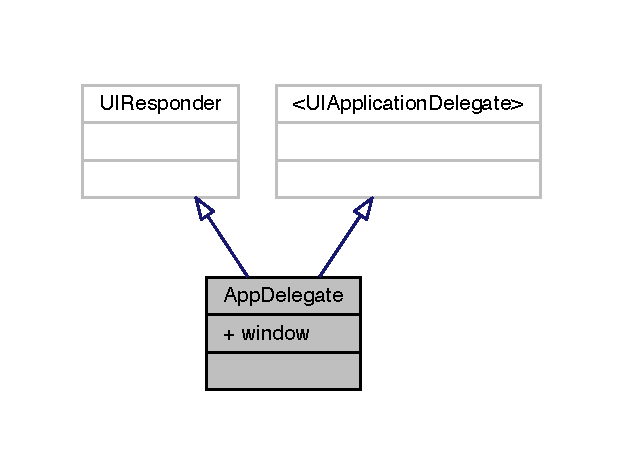
\includegraphics[width=299pt]{interface_app_delegate__inherit__graph}
\end{center}
\end{figure}


Collaboration diagram for App\-Delegate\-:\nopagebreak
\begin{figure}[H]
\begin{center}
\leavevmode
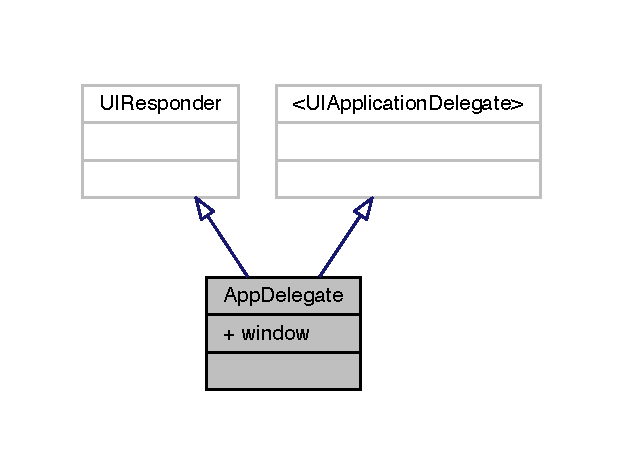
\includegraphics[width=299pt]{interface_app_delegate__coll__graph}
\end{center}
\end{figure}
\subsection*{Properties}
\begin{DoxyCompactItemize}
\item 
\hypertarget{interface_app_delegate_acf48ac24125e688cac1a85445cd7fac2}{U\-I\-Window $\ast$ {\bfseries window}}\label{interface_app_delegate_acf48ac24125e688cac1a85445cd7fac2}

\end{DoxyCompactItemize}


The documentation for this class was generated from the following file\-:\begin{DoxyCompactItemize}
\item 
Pack\-Manager/App\-Delegate.\-h\end{DoxyCompactItemize}

\hypertarget{interface_destination}{\section{Destination Class Reference}
\label{interface_destination}\index{Destination@{Destination}}
}


{\ttfamily \#import $<$Destination.\-h$>$}



Inheritance diagram for Destination\-:
\nopagebreak
\begin{figure}[H]
\begin{center}
\leavevmode
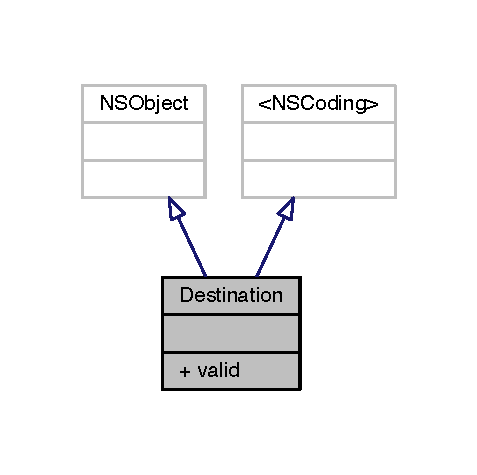
\includegraphics[width=229pt]{interface_destination__inherit__graph}
\end{center}
\end{figure}


Collaboration diagram for Destination\-:
\nopagebreak
\begin{figure}[H]
\begin{center}
\leavevmode
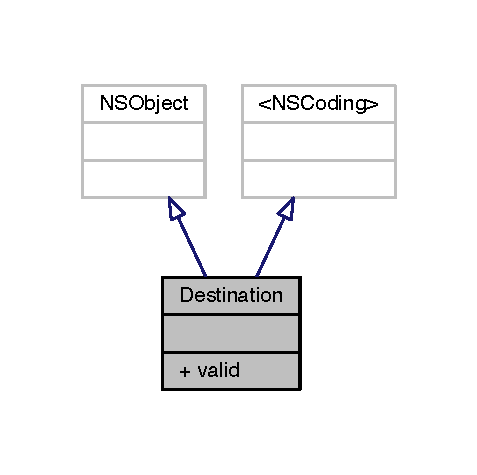
\includegraphics[width=229pt]{interface_destination__coll__graph}
\end{center}
\end{figure}
\subsection*{Instance Methods}
\begin{DoxyCompactItemize}
\item 
(B\-O\-O\-L) -\/ \hyperlink{interface_destination_ae33ba4170b0e92f1b94ae6f21f5c3dbb}{valid}
\item 
(B\-O\-O\-L) -\/ \hyperlink{interface_destination_a906246f5d15394fa5d8f5fee672537e1}{is\-Valid\-Z\-I\-P\-:}
\end{DoxyCompactItemize}
\subsection*{Properties}
\begin{DoxyCompactItemize}
\item 
N\-S\-Integer \hyperlink{interface_destination_a83a4c63fc216c137f29aadaa4be1fda2}{duration}
\item 
N\-S\-Integer \hyperlink{interface_destination_ac3fa98f68bc95bf00852743e1b3d3f9a}{zip}
\item 
\hypertarget{interface_destination_ab21be07a3201646736da1899501cb46c}{N\-S\-String $\ast$ {\bfseries name}}\label{interface_destination_ab21be07a3201646736da1899501cb46c}

\item 
\hypertarget{interface_destination_af6e9f0de5a758bd0572864f45a5040e6}{C\-G\-Float {\bfseries lat}}\label{interface_destination_af6e9f0de5a758bd0572864f45a5040e6}

\item 
\hypertarget{interface_destination_ad9d95f6874e1ff4f73ea4f69c60c093a}{C\-G\-Float {\bfseries lon}}\label{interface_destination_ad9d95f6874e1ff4f73ea4f69c60c093a}

\end{DoxyCompactItemize}


\subsection{Detailed Description}
Adds some convenience methods to the \hyperlink{interface_destination}{Destination} class

\hyperlink{interface_destination}{Destination} class maintains stops for a trip. It is responsible for maintaining destination location and duration of stay at said location. 

\subsection{Method Documentation}
\hypertarget{interface_destination_a906246f5d15394fa5d8f5fee672537e1}{\index{Destination@{Destination}!is\-Valid\-Z\-I\-P\-:@{is\-Valid\-Z\-I\-P\-:}}
\index{is\-Valid\-Z\-I\-P\-:@{is\-Valid\-Z\-I\-P\-:}!Destination@{Destination}}
\subsubsection[{is\-Valid\-Z\-I\-P\-:}]{\setlength{\rightskip}{0pt plus 5cm}-\/ (B\-O\-O\-L) is\-Valid\-Z\-I\-P\-: 
\begin{DoxyParamCaption}
\item[{(N\-S\-Integer)}]{zip}
\end{DoxyParamCaption}
}}\label{interface_destination_a906246f5d15394fa5d8f5fee672537e1}
Method to validate given Z\-I\-P code. 
\begin{DoxyParams}{Parameters}
{\em zip} & Z\-I\-P code in question \\
\hline
\end{DoxyParams}
\begin{DoxyReturn}{Returns}
T\-R\-U\-E if zip is a valid zip code, false otherwise. 
\end{DoxyReturn}
\hypertarget{interface_destination_ae33ba4170b0e92f1b94ae6f21f5c3dbb}{\index{Destination@{Destination}!valid@{valid}}
\index{valid@{valid}!Destination@{Destination}}
\subsubsection[{valid}]{\setlength{\rightskip}{0pt plus 5cm}-\/ (B\-O\-O\-L) valid 
\begin{DoxyParamCaption}
{}
\end{DoxyParamCaption}
}}\label{interface_destination_ae33ba4170b0e92f1b94ae6f21f5c3dbb}
Tests to see if a destination is a valid location  returns T\-R\-U\-E if location is a valid place (i.\-e. it exists), otherwise returns F\-A\-L\-S\-E 

\subsection{Property Documentation}
\hypertarget{interface_destination_a83a4c63fc216c137f29aadaa4be1fda2}{\index{Destination@{Destination}!duration@{duration}}
\index{duration@{duration}!Destination@{Destination}}
\subsubsection[{duration}]{\setlength{\rightskip}{0pt plus 5cm}-\/ (N\-S\-Integer) duration\hspace{0.3cm}{\ttfamily [read]}, {\ttfamily [write]}, {\ttfamily [nonatomic]}, {\ttfamily [assign]}}}\label{interface_destination_a83a4c63fc216c137f29aadaa4be1fda2}
Duration of the trip, positive value \hypertarget{interface_destination_ac3fa98f68bc95bf00852743e1b3d3f9a}{\index{Destination@{Destination}!zip@{zip}}
\index{zip@{zip}!Destination@{Destination}}
\subsubsection[{zip}]{\setlength{\rightskip}{0pt plus 5cm}-\/ (N\-S\-Integer) zip\hspace{0.3cm}{\ttfamily [read]}, {\ttfamily [write]}, {\ttfamily [nonatomic]}, {\ttfamily [assign]}}}\label{interface_destination_ac3fa98f68bc95bf00852743e1b3d3f9a}
Z\-I\-P Code for the given location 

The documentation for this class was generated from the following files\-:\begin{DoxyCompactItemize}
\item 
Pack\-Manager/Destination.\-h\item 
Pack\-Manager/Destination.\-m\end{DoxyCompactItemize}

\hypertarget{interface_layered_right_detail_cell}{\section{Layered\-Right\-Detail\-Cell Class Reference}
\label{interface_layered_right_detail_cell}\index{Layered\-Right\-Detail\-Cell@{Layered\-Right\-Detail\-Cell}}
}


Inheritance diagram for Layered\-Right\-Detail\-Cell\-:\nopagebreak
\begin{figure}[H]
\begin{center}
\leavevmode
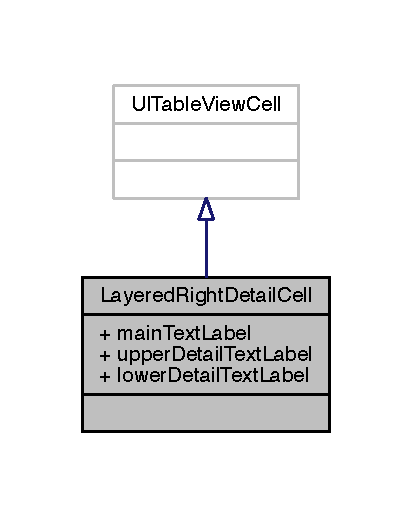
\includegraphics[width=198pt]{interface_layered_right_detail_cell__inherit__graph}
\end{center}
\end{figure}


Collaboration diagram for Layered\-Right\-Detail\-Cell\-:\nopagebreak
\begin{figure}[H]
\begin{center}
\leavevmode
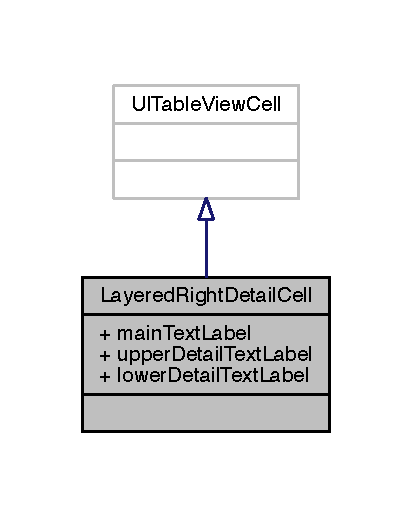
\includegraphics[width=198pt]{interface_layered_right_detail_cell__coll__graph}
\end{center}
\end{figure}
\subsection*{Properties}
\begin{DoxyCompactItemize}
\item 
\hypertarget{interface_layered_right_detail_cell_aabc0589a423bde3b49a53a9d4be5277b}{I\-B\-Outlet U\-I\-Label $\ast$ {\bfseries main\-Text\-Label}}\label{interface_layered_right_detail_cell_aabc0589a423bde3b49a53a9d4be5277b}

\item 
\hypertarget{interface_layered_right_detail_cell_a640825f6998623ef2d1c17589daaf877}{I\-B\-Outlet U\-I\-Label $\ast$ {\bfseries upper\-Detail\-Text\-Label}}\label{interface_layered_right_detail_cell_a640825f6998623ef2d1c17589daaf877}

\item 
\hypertarget{interface_layered_right_detail_cell_a91a30bbf1dbe60d1871978b54daf8520}{I\-B\-Outlet U\-I\-Label $\ast$ {\bfseries lower\-Detail\-Text\-Label}}\label{interface_layered_right_detail_cell_a91a30bbf1dbe60d1871978b54daf8520}

\end{DoxyCompactItemize}


The documentation for this class was generated from the following file\-:\begin{DoxyCompactItemize}
\item 
Pack\-Manager/Layered\-Right\-Detail\-Cell.\-h\end{DoxyCompactItemize}

\hypertarget{interface_new_trip_view_controller}{\section{New\-Trip\-View\-Controller Class Reference}
\label{interface_new_trip_view_controller}\index{New\-Trip\-View\-Controller@{New\-Trip\-View\-Controller}}
}


Inheritance diagram for New\-Trip\-View\-Controller\-:\nopagebreak
\begin{figure}[H]
\begin{center}
\leavevmode
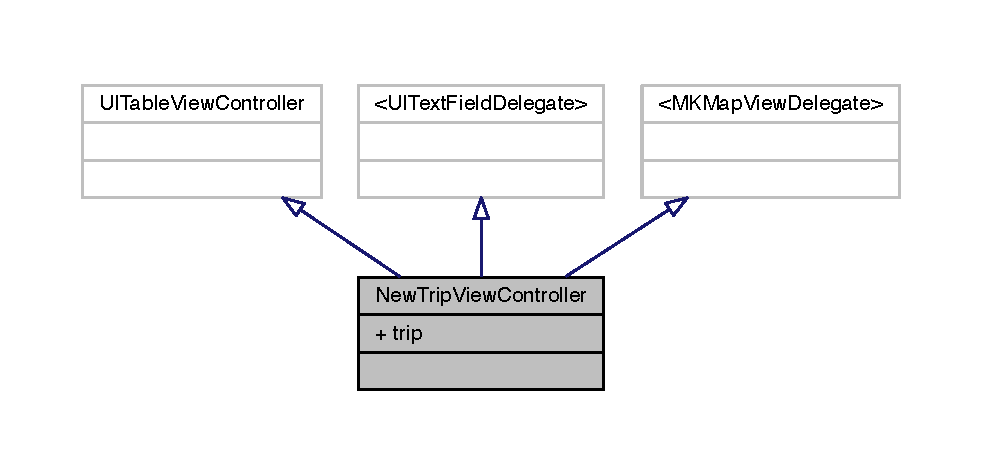
\includegraphics[width=196pt]{interface_new_trip_view_controller__inherit__graph}
\end{center}
\end{figure}


Collaboration diagram for New\-Trip\-View\-Controller\-:\nopagebreak
\begin{figure}[H]
\begin{center}
\leavevmode
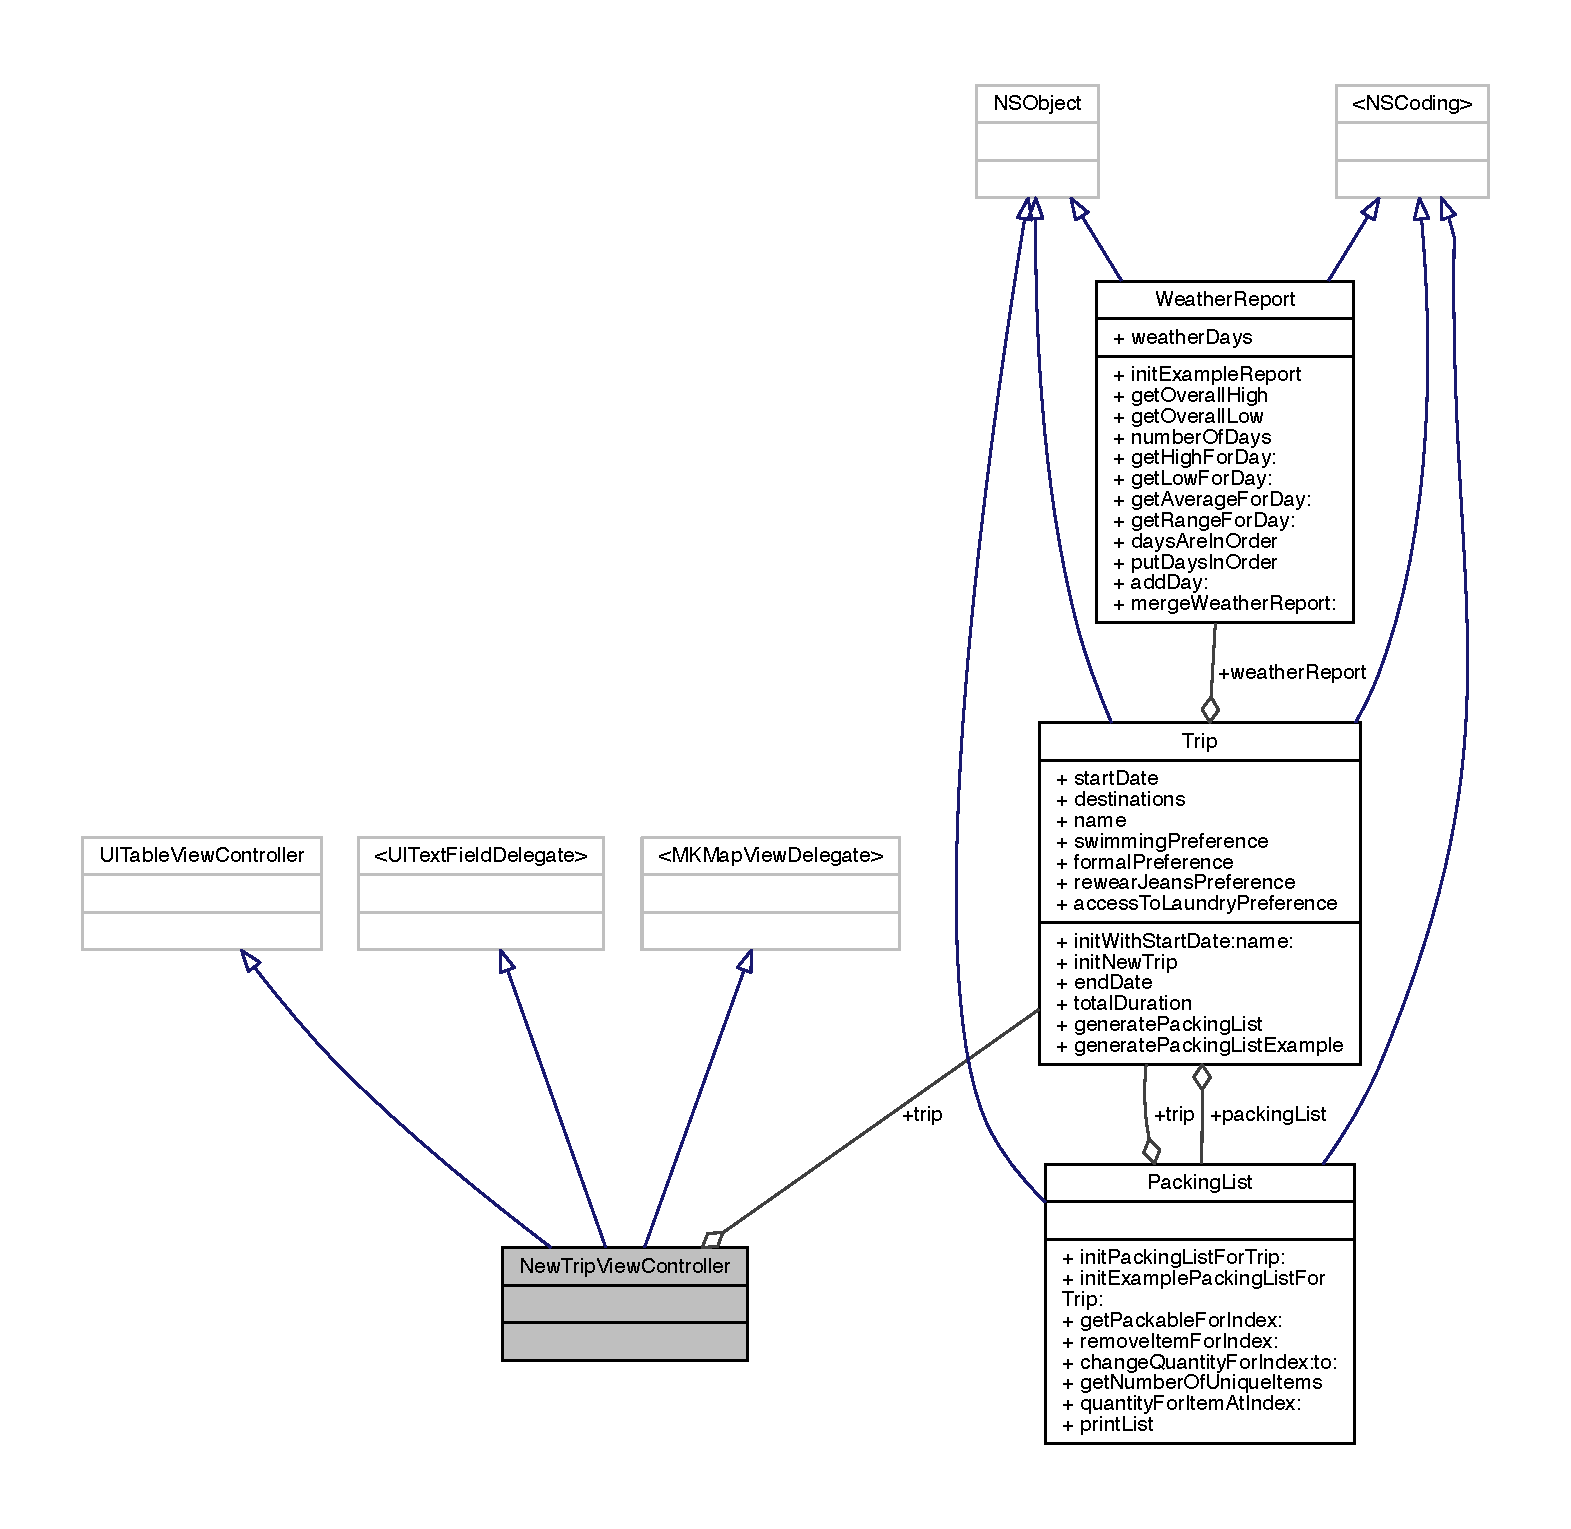
\includegraphics[width=196pt]{interface_new_trip_view_controller__coll__graph}
\end{center}
\end{figure}


The documentation for this class was generated from the following file\-:\begin{DoxyCompactItemize}
\item 
Pack\-Manager/New\-Trip\-View\-Controller.\-h\end{DoxyCompactItemize}

\hypertarget{category_new_trip_view_controller_07_08}{\section{New\-Trip\-View\-Controller() Category Reference}
\label{category_new_trip_view_controller_07_08}\index{New\-Trip\-View\-Controller()@{New\-Trip\-View\-Controller()}}
}


Collaboration diagram for New\-Trip\-View\-Controller()\-:\nopagebreak
\begin{figure}[H]
\begin{center}
\leavevmode
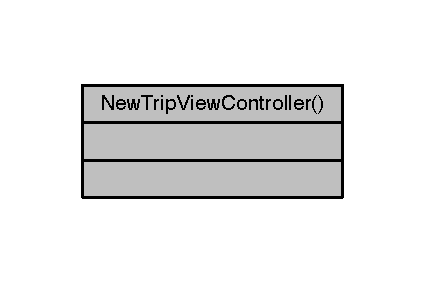
\includegraphics[width=238pt]{category_new_trip_view_controller_07_08__coll__graph}
\end{center}
\end{figure}
\subsection*{Instance Methods}
\begin{DoxyCompactItemize}
\item 
\hypertarget{category_new_trip_view_controller_07_08_a13a1e787f7bba2412b8254a2c5552863}{(I\-B\-Action) -\/ {\bfseries start\-Date\-Picked\-:}}\label{category_new_trip_view_controller_07_08_a13a1e787f7bba2412b8254a2c5552863}

\item 
\hypertarget{category_new_trip_view_controller_07_08_ad2bc2e48e85627ef5d02f21569694c15}{(I\-B\-Action) -\/ {\bfseries add\-Stop\-Button\-Press\-:}}\label{category_new_trip_view_controller_07_08_ad2bc2e48e85627ef5d02f21569694c15}

\end{DoxyCompactItemize}
\subsection*{Properties}
\begin{DoxyCompactItemize}
\item 
\hypertarget{category_new_trip_view_controller_07_08_a4de5831400f9c1599152b534ca83a801}{I\-B\-Outlet U\-I\-Button $\ast$ {\bfseries add\-Stop\-Button}}\label{category_new_trip_view_controller_07_08_a4de5831400f9c1599152b534ca83a801}

\item 
\hypertarget{category_new_trip_view_controller_07_08_abbce0a1b0d8abce963ced44be5f6cd33}{I\-B\-Outlet U\-I\-Button $\ast$ {\bfseries generate\-List\-Button}}\label{category_new_trip_view_controller_07_08_abbce0a1b0d8abce963ced44be5f6cd33}

\item 
\hypertarget{category_new_trip_view_controller_07_08_a21eb151ed2a52e4bcf751cd72f57233c}{I\-B\-Outlet U\-I\-Text\-Field $\ast$ {\bfseries trip\-Name\-Text\-Field}}\label{category_new_trip_view_controller_07_08_a21eb151ed2a52e4bcf751cd72f57233c}

\item 
\hypertarget{category_new_trip_view_controller_07_08_ac36b7787abef9c7a1fe648c471a8a8ee}{I\-B\-Outlet U\-I\-Date\-Picker $\ast$ {\bfseries start\-Date\-Picker}}\label{category_new_trip_view_controller_07_08_ac36b7787abef9c7a1fe648c471a8a8ee}

\item 
\hypertarget{category_new_trip_view_controller_07_08_a9e87d61abcadfeaca563b76bfa4a78fa}{I\-B\-Outlet U\-I\-Text\-Field $\ast$ {\bfseries curr\-Location\-Text\-Field}}\label{category_new_trip_view_controller_07_08_a9e87d61abcadfeaca563b76bfa4a78fa}

\item 
\hypertarget{category_new_trip_view_controller_07_08_a77f519b5859833202b99a0234f6835eb}{I\-B\-Outlet U\-I\-Table\-View $\ast$ {\bfseries location\-Suggestions\-Table\-View}}\label{category_new_trip_view_controller_07_08_a77f519b5859833202b99a0234f6835eb}

\item 
\hypertarget{category_new_trip_view_controller_07_08_a8e98bb0c2df9d96bcf86193f0c116f79}{I\-B\-Outlet M\-K\-Map\-View $\ast$ {\bfseries map\-View}}\label{category_new_trip_view_controller_07_08_a8e98bb0c2df9d96bcf86193f0c116f79}

\item 
\hypertarget{category_new_trip_view_controller_07_08_a4149be533fd16b7d618aeb07eff1821c}{I\-B\-Outlet U\-I\-Text\-Field $\ast$ {\bfseries curr\-Duration\-Text\-Field}}\label{category_new_trip_view_controller_07_08_a4149be533fd16b7d618aeb07eff1821c}

\end{DoxyCompactItemize}


The documentation for this category was generated from the following file\-:\begin{DoxyCompactItemize}
\item 
Pack\-Manager/New\-Trip\-View\-Controller.\-m\end{DoxyCompactItemize}

\hypertarget{interface_packable}{\section{Packable Class Reference}
\label{interface_packable}\index{Packable@{Packable}}
}


Inheritance diagram for Packable\-:\nopagebreak
\begin{figure}[H]
\begin{center}
\leavevmode
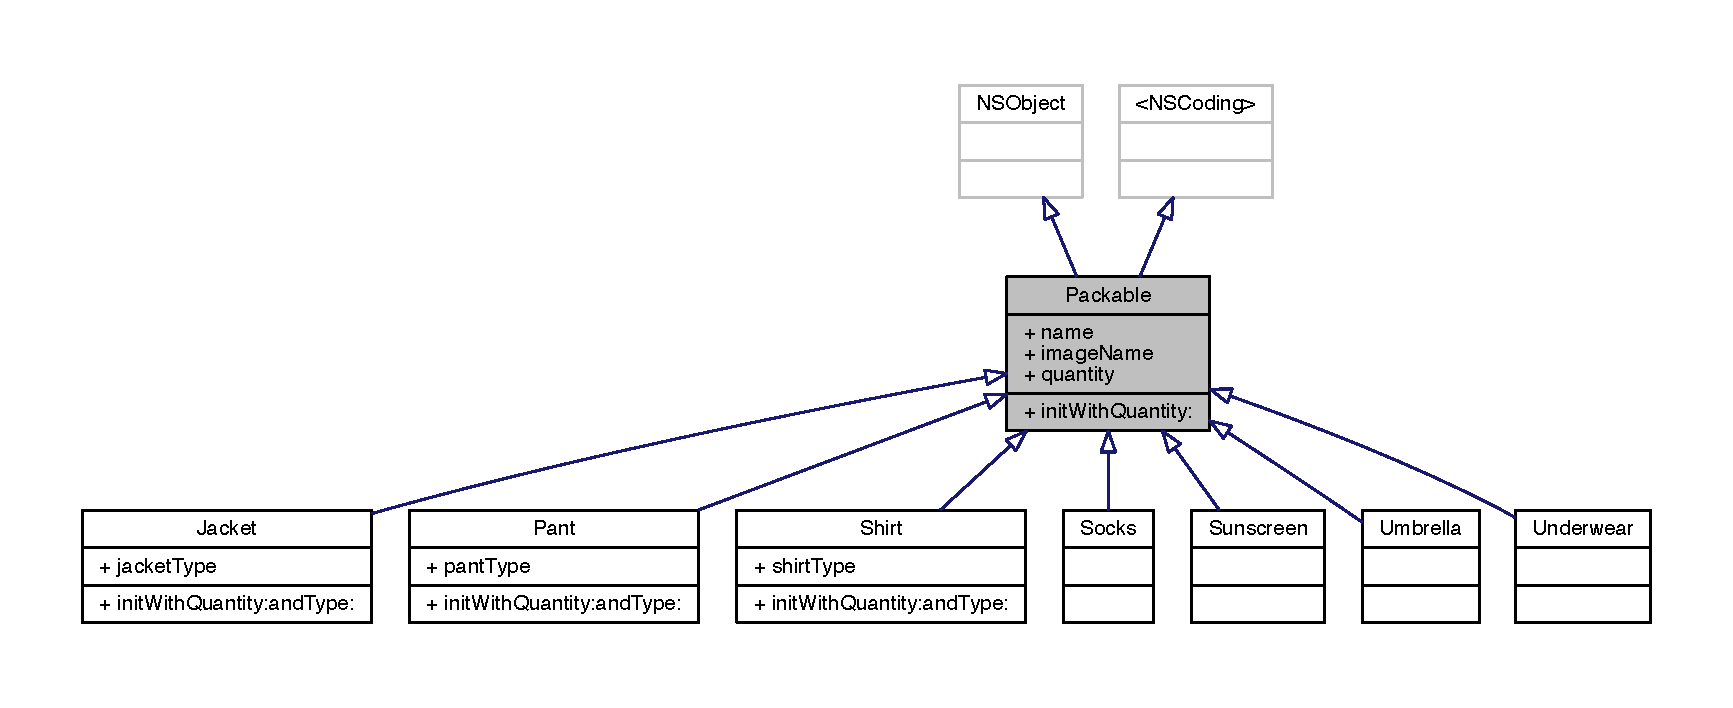
\includegraphics[width=138pt]{interface_packable__inherit__graph}
\end{center}
\end{figure}


Collaboration diagram for Packable\-:\nopagebreak
\begin{figure}[H]
\begin{center}
\leavevmode
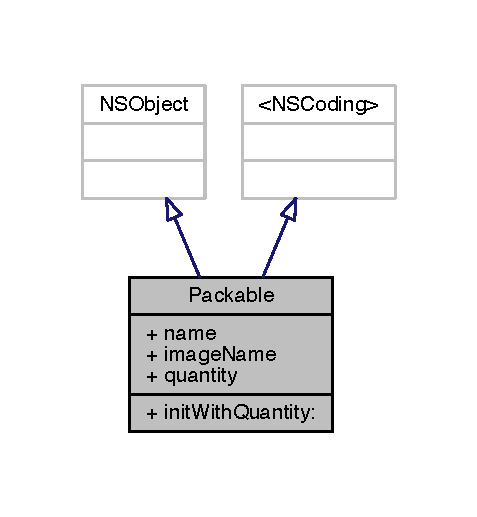
\includegraphics[width=138pt]{interface_packable__coll__graph}
\end{center}
\end{figure}
\subsection*{Properties}
\begin{DoxyCompactItemize}
\item 
\hypertarget{interface_packable_ac796b857c15e96bfe0cab64d4f855b8d}{N\-S\-String $\ast$ {\bfseries name}}\label{interface_packable_ac796b857c15e96bfe0cab64d4f855b8d}

\item 
\hypertarget{interface_packable_a1bcccd6d856e10d677a6ba2c86f87768}{N\-S\-Integer {\bfseries quantity}}\label{interface_packable_a1bcccd6d856e10d677a6ba2c86f87768}

\end{DoxyCompactItemize}


The documentation for this class was generated from the following file\-:\begin{DoxyCompactItemize}
\item 
Pack\-Manager/Packable.\-h\end{DoxyCompactItemize}

\hypertarget{interface_packing_list}{\section{Packing\-List Class Reference}
\label{interface_packing_list}\index{Packing\-List@{Packing\-List}}
}


{\ttfamily \#import $<$Packing\-List.\-h$>$}



Inheritance diagram for Packing\-List\-:\nopagebreak
\begin{figure}[H]
\begin{center}
\leavevmode
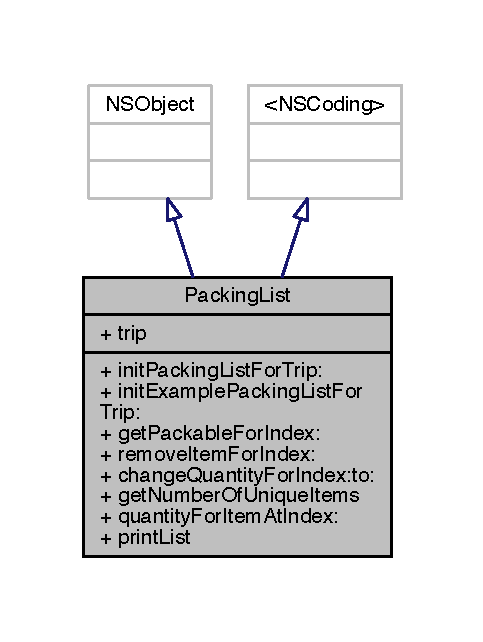
\includegraphics[width=232pt]{interface_packing_list__inherit__graph}
\end{center}
\end{figure}


Collaboration diagram for Packing\-List\-:
\nopagebreak
\begin{figure}[H]
\begin{center}
\leavevmode
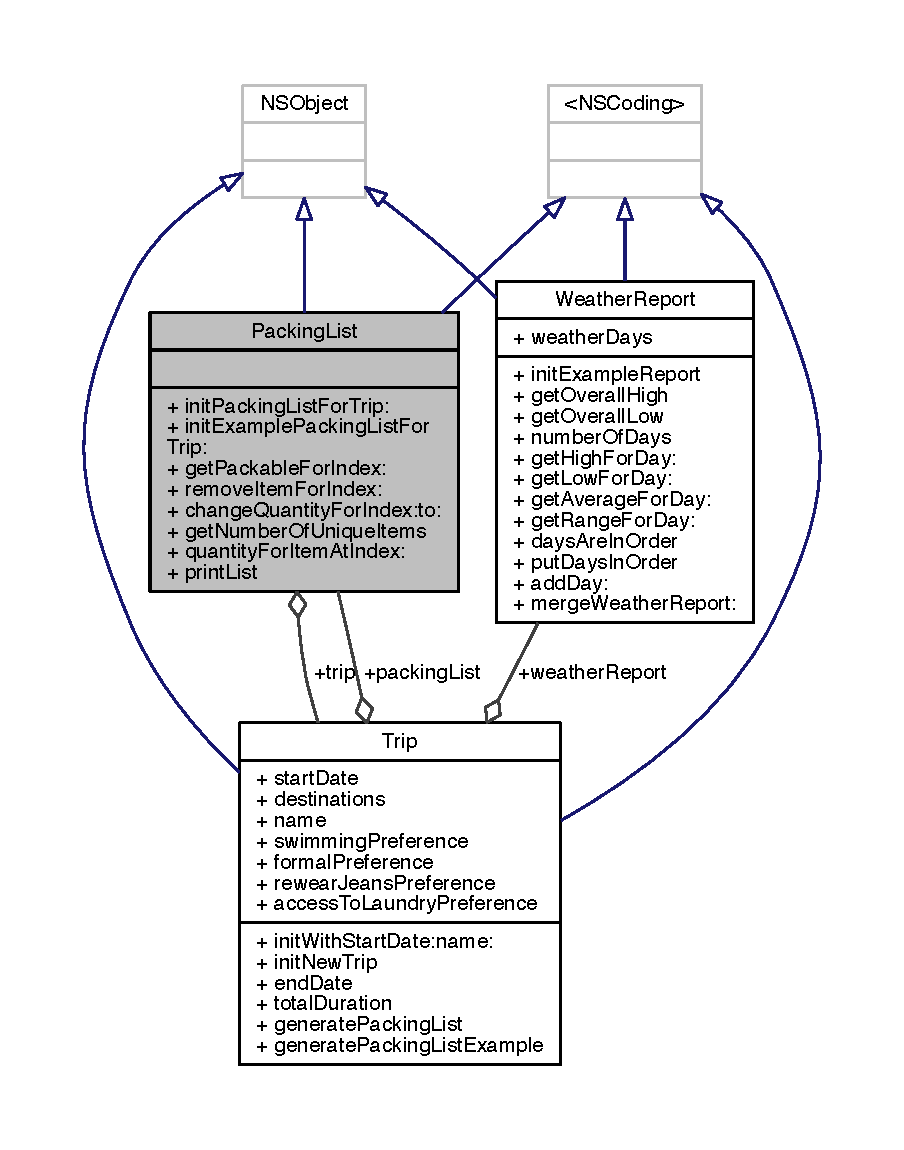
\includegraphics[width=350pt]{interface_packing_list__coll__graph}
\end{center}
\end{figure}
\subsection*{Instance Methods}
\begin{DoxyCompactItemize}
\item 
(instancetype) -\/ \hyperlink{interface_packing_list_ad2a2047f09bda181d360593acb068cab}{init\-Packing\-List\-For\-Trip\-:}
\item 
(instancetype) -\/ \hyperlink{interface_packing_list_a1a06132f16892f9379ded65f2365362b}{init\-Example\-Packing\-List\-For\-Trip\-:}
\item 
(\hyperlink{interface_packable}{Packable} $\ast$) -\/ \hyperlink{interface_packing_list_a09a1d6b99216336d3de2f1d39983e4fd}{get\-Packable\-For\-Index\-:}
\item 
(void) -\/ \hyperlink{interface_packing_list_a0eeb9568c172bfc8ff5194ea9b31dc40}{remove\-Item\-For\-Index\-:}
\item 
(void) -\/ \hyperlink{interface_packing_list_ac17f7681dfe6d6fd48610412c6c81d6a}{change\-Quantity\-For\-Index\-:to\-:}
\item 
(N\-S\-Integer) -\/ \hyperlink{interface_packing_list_abc46addde8828e6e414100851eac731e}{get\-Number\-Of\-Unique\-Items}
\item 
(N\-S\-Integer) -\/ \hyperlink{interface_packing_list_a4b7a74a055c78ad2c84365b9fd2567cd}{quantity\-For\-Item\-At\-Index\-:}
\item 
(void) -\/ \hyperlink{interface_packing_list_a91482348b38c1a7762a08e914306714f}{print\-List}
\end{DoxyCompactItemize}
\subsection*{Properties}
\begin{DoxyCompactItemize}
\item 
\hyperlink{interface_trip}{Trip} $\ast$ \hyperlink{interface_packing_list_a12ca48b216cfbdc18f1e34849d17adb4}{trip}
\end{DoxyCompactItemize}


\subsection{Detailed Description}
Class that represents a list of packing items and adds some convenience methods 

\subsection{Method Documentation}
\hypertarget{interface_packing_list_ac17f7681dfe6d6fd48610412c6c81d6a}{\index{Packing\-List@{Packing\-List}!change\-Quantity\-For\-Index\-:to\-:@{change\-Quantity\-For\-Index\-:to\-:}}
\index{change\-Quantity\-For\-Index\-:to\-:@{change\-Quantity\-For\-Index\-:to\-:}!PackingList@{Packing\-List}}
\subsubsection[{change\-Quantity\-For\-Index\-:to\-:}]{\setlength{\rightskip}{0pt plus 5cm}-\/ (void) change\-Quantity\-For\-Index\-: 
\begin{DoxyParamCaption}
\item[{(N\-S\-Integer)}]{index}
\item[{to:(N\-S\-Integer)}]{q}
\end{DoxyParamCaption}
}}\label{interface_packing_list_ac17f7681dfe6d6fd48610412c6c81d6a}
Updates the quantiy for the packable at a certain index 
\begin{DoxyParams}{Parameters}
{\em index} & The index of a packable in the \hyperlink{interface_packing_list}{Packing\-List} you wish to change \\
\hline
{\em q} & The updated quantity for the packable \\
\hline
\end{DoxyParams}
\hypertarget{interface_packing_list_abc46addde8828e6e414100851eac731e}{\index{Packing\-List@{Packing\-List}!get\-Number\-Of\-Unique\-Items@{get\-Number\-Of\-Unique\-Items}}
\index{get\-Number\-Of\-Unique\-Items@{get\-Number\-Of\-Unique\-Items}!PackingList@{Packing\-List}}
\subsubsection[{get\-Number\-Of\-Unique\-Items}]{\setlength{\rightskip}{0pt plus 5cm}-\/ (N\-S\-Integer) get\-Number\-Of\-Unique\-Items 
\begin{DoxyParamCaption}
{}
\end{DoxyParamCaption}
}}\label{interface_packing_list_abc46addde8828e6e414100851eac731e}
Returns number of different types of items For instance, if the list has 3 shirts and 5 pants, this will return 2 (shirts, pants) \begin{DoxyReturn}{Returns}
an integer representing the number of unique items 
\end{DoxyReturn}
\hypertarget{interface_packing_list_a09a1d6b99216336d3de2f1d39983e4fd}{\index{Packing\-List@{Packing\-List}!get\-Packable\-For\-Index\-:@{get\-Packable\-For\-Index\-:}}
\index{get\-Packable\-For\-Index\-:@{get\-Packable\-For\-Index\-:}!PackingList@{Packing\-List}}
\subsubsection[{get\-Packable\-For\-Index\-:}]{\setlength{\rightskip}{0pt plus 5cm}-\/ ({\bf Packable} $\ast$) get\-Packable\-For\-Index\-: 
\begin{DoxyParamCaption}
\item[{(N\-S\-Integer)}]{index}
\end{DoxyParamCaption}
}}\label{interface_packing_list_a09a1d6b99216336d3de2f1d39983e4fd}
Returns a packable item that as at the given index in the \hyperlink{interface_packing_list}{Packing\-List} object 
\begin{DoxyParams}{Parameters}
{\em index} & The index of a packable in the \hyperlink{interface_packing_list}{Packing\-List} you wish to retrieve \\
\hline
\end{DoxyParams}
\begin{DoxyReturn}{Returns}
a packable item at the given index 
\end{DoxyReturn}
\hypertarget{interface_packing_list_a1a06132f16892f9379ded65f2365362b}{\index{Packing\-List@{Packing\-List}!init\-Example\-Packing\-List\-For\-Trip\-:@{init\-Example\-Packing\-List\-For\-Trip\-:}}
\index{init\-Example\-Packing\-List\-For\-Trip\-:@{init\-Example\-Packing\-List\-For\-Trip\-:}!PackingList@{Packing\-List}}
\subsubsection[{init\-Example\-Packing\-List\-For\-Trip\-:}]{\setlength{\rightskip}{0pt plus 5cm}-\/ (instancetype) init\-Example\-Packing\-List\-For\-Trip\-: 
\begin{DoxyParamCaption}
\item[{({\bf Trip} $\ast$)}]{trip}
\end{DoxyParamCaption}
}}\label{interface_packing_list_a1a06132f16892f9379ded65f2365362b}
Initialize a new demo packing list. This method always returns the exact same packing list.  trip The trip this packing list is attributed to \hypertarget{interface_packing_list_ad2a2047f09bda181d360593acb068cab}{\index{Packing\-List@{Packing\-List}!init\-Packing\-List\-For\-Trip\-:@{init\-Packing\-List\-For\-Trip\-:}}
\index{init\-Packing\-List\-For\-Trip\-:@{init\-Packing\-List\-For\-Trip\-:}!PackingList@{Packing\-List}}
\subsubsection[{init\-Packing\-List\-For\-Trip\-:}]{\setlength{\rightskip}{0pt plus 5cm}-\/ (instancetype) init\-Packing\-List\-For\-Trip\-: 
\begin{DoxyParamCaption}
\item[{({\bf Trip} $\ast$)}]{trip}
\end{DoxyParamCaption}
}}\label{interface_packing_list_ad2a2047f09bda181d360593acb068cab}
Initialize a new \hyperlink{interface_packing_list}{Packing\-List} object 
\begin{DoxyParams}{Parameters}
{\em trip} & The trip the packing list is for \\
\hline
\end{DoxyParams}
\begin{DoxyReturn}{Returns}
a newly intialized object 
\end{DoxyReturn}
\hypertarget{interface_packing_list_a91482348b38c1a7762a08e914306714f}{\index{Packing\-List@{Packing\-List}!print\-List@{print\-List}}
\index{print\-List@{print\-List}!PackingList@{Packing\-List}}
\subsubsection[{print\-List}]{\setlength{\rightskip}{0pt plus 5cm}-\/ (void) print\-List 
\begin{DoxyParamCaption}
{}
\end{DoxyParamCaption}
}}\label{interface_packing_list_a91482348b38c1a7762a08e914306714f}
Information Hiding! This class will convert it's items' names into strings for you 
\begin{DoxyParams}{Parameters}
{\em item} & A packing item \\
\hline
\end{DoxyParams}
\begin{DoxyReturn}{Returns}
a string representation of the given item Used for testing, this function will print out the packing list to the console. 
\end{DoxyReturn}
\hypertarget{interface_packing_list_a4b7a74a055c78ad2c84365b9fd2567cd}{\index{Packing\-List@{Packing\-List}!quantity\-For\-Item\-At\-Index\-:@{quantity\-For\-Item\-At\-Index\-:}}
\index{quantity\-For\-Item\-At\-Index\-:@{quantity\-For\-Item\-At\-Index\-:}!PackingList@{Packing\-List}}
\subsubsection[{quantity\-For\-Item\-At\-Index\-:}]{\setlength{\rightskip}{0pt plus 5cm}-\/ (N\-S\-Integer) quantity\-For\-Item\-At\-Index\-: 
\begin{DoxyParamCaption}
\item[{(N\-S\-Integer)}]{index}
\end{DoxyParamCaption}
}}\label{interface_packing_list_a4b7a74a055c78ad2c84365b9fd2567cd}
Returns the number of items at a specific index For instance, 5 socks at index 6. 
\begin{DoxyParams}{Parameters}
{\em index} & The index to examine \\
\hline
\end{DoxyParams}
\begin{DoxyReturn}{Returns}
an integer representing the quantity of items at given index 
\end{DoxyReturn}
\hypertarget{interface_packing_list_a0eeb9568c172bfc8ff5194ea9b31dc40}{\index{Packing\-List@{Packing\-List}!remove\-Item\-For\-Index\-:@{remove\-Item\-For\-Index\-:}}
\index{remove\-Item\-For\-Index\-:@{remove\-Item\-For\-Index\-:}!PackingList@{Packing\-List}}
\subsubsection[{remove\-Item\-For\-Index\-:}]{\setlength{\rightskip}{0pt plus 5cm}-\/ (void) remove\-Item\-For\-Index\-: 
\begin{DoxyParamCaption}
\item[{(N\-S\-Integer)}]{index}
\end{DoxyParamCaption}
}}\label{interface_packing_list_a0eeb9568c172bfc8ff5194ea9b31dc40}
Deletes a packing list item from the list 
\begin{DoxyParams}{Parameters}
{\em index} & The index of a packable in the \hyperlink{interface_packing_list}{Packing\-List} you wish to delete \\
\hline
\end{DoxyParams}


\subsection{Property Documentation}
\hypertarget{interface_packing_list_a12ca48b216cfbdc18f1e34849d17adb4}{\index{Packing\-List@{Packing\-List}!trip@{trip}}
\index{trip@{trip}!PackingList@{Packing\-List}}
\subsubsection[{trip}]{\setlength{\rightskip}{0pt plus 5cm}-\/ ({\bf Trip}$\ast$) trip\hspace{0.3cm}{\ttfamily [read]}, {\ttfamily [write]}, {\ttfamily [nonatomic]}, {\ttfamily [strong]}}}\label{interface_packing_list_a12ca48b216cfbdc18f1e34849d17adb4}
\hyperlink{interface_trip}{Trip} object that this packing list refers to. 

The documentation for this class was generated from the following files\-:\begin{DoxyCompactItemize}
\item 
Pack\-Manager/Packing\-List.\-h\item 
Pack\-Manager/Packing\-List.\-m\end{DoxyCompactItemize}

\hypertarget{category_packing_list_07_08}{\section{Packing\-List() Category Reference}
\label{category_packing_list_07_08}\index{Packing\-List()@{Packing\-List()}}
}


Collaboration diagram for Packing\-List()\-:\nopagebreak
\begin{figure}[H]
\begin{center}
\leavevmode
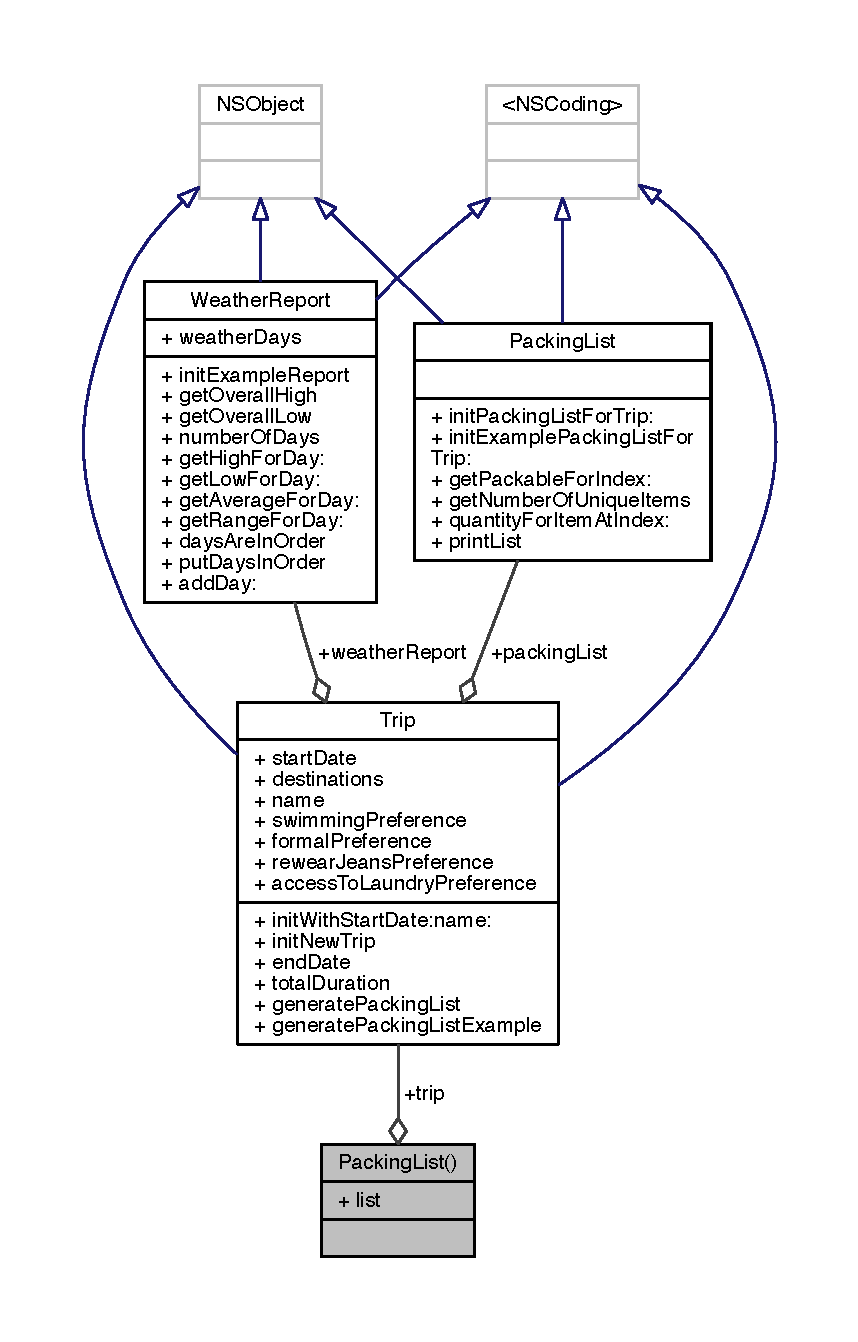
\includegraphics[width=350pt]{category_packing_list_07_08__coll__graph}
\end{center}
\end{figure}
\subsection*{Properties}
\begin{DoxyCompactItemize}
\item 
\hypertarget{category_packing_list_07_08_a292ad22790d68f0529063efcb9c043f4}{N\-S\-Mutable\-Array $\ast$ {\bfseries list}}\label{category_packing_list_07_08_a292ad22790d68f0529063efcb9c043f4}

\item 
\hypertarget{category_packing_list_07_08_a37b182ab8a91dce0cff8799c1c2a5c64}{\hyperlink{interface_trip}{Trip} $\ast$ {\bfseries trip}}\label{category_packing_list_07_08_a37b182ab8a91dce0cff8799c1c2a5c64}

\end{DoxyCompactItemize}


The documentation for this category was generated from the following file\-:\begin{DoxyCompactItemize}
\item 
Pack\-Manager/Packing\-List.\-m\end{DoxyCompactItemize}

\hypertarget{class_packing_list_item_cell}{\section{Packing\-List\-Item\-Cell Class Reference}
\label{class_packing_list_item_cell}\index{Packing\-List\-Item\-Cell@{Packing\-List\-Item\-Cell}}
}


Collaboration diagram for Packing\-List\-Item\-Cell\-:\nopagebreak
\begin{figure}[H]
\begin{center}
\leavevmode
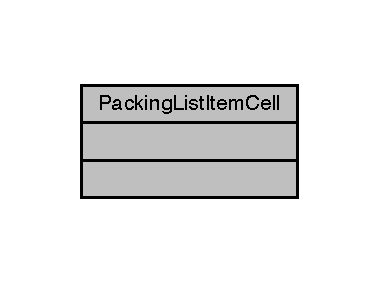
\includegraphics[width=182pt]{class_packing_list_item_cell__coll__graph}
\end{center}
\end{figure}


The documentation for this class was generated from the following file\-:\begin{DoxyCompactItemize}
\item 
Pack\-Manager/Packing\-List\-Item\-Cell.\-m\end{DoxyCompactItemize}

\hypertarget{interface_packing_list_view_controller}{\section{Packing\-List\-View\-Controller Class Reference}
\label{interface_packing_list_view_controller}\index{Packing\-List\-View\-Controller@{Packing\-List\-View\-Controller}}
}


Inheritance diagram for Packing\-List\-View\-Controller\-:\nopagebreak
\begin{figure}[H]
\begin{center}
\leavevmode
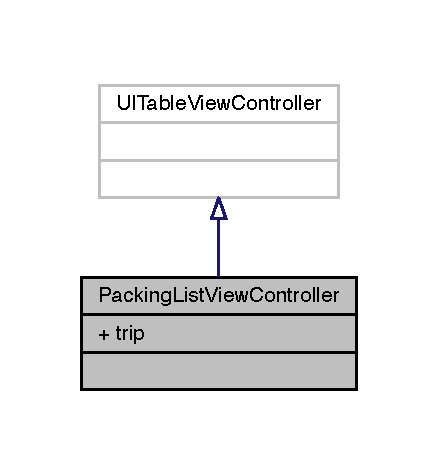
\includegraphics[width=210pt]{interface_packing_list_view_controller__inherit__graph}
\end{center}
\end{figure}


Collaboration diagram for Packing\-List\-View\-Controller\-:\nopagebreak
\begin{figure}[H]
\begin{center}
\leavevmode
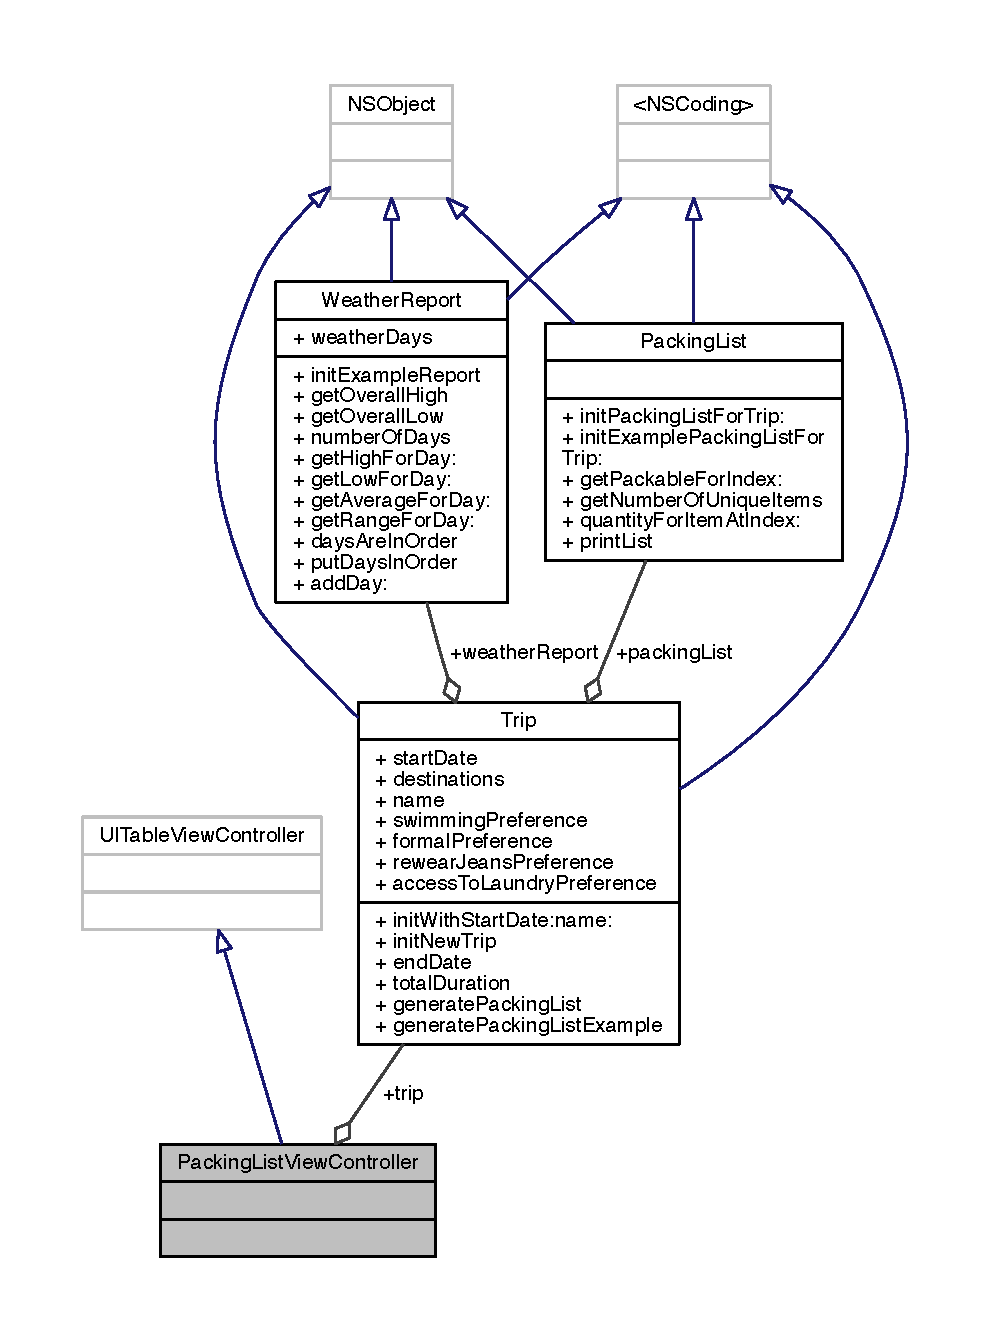
\includegraphics[width=350pt]{interface_packing_list_view_controller__coll__graph}
\end{center}
\end{figure}
\subsection*{Properties}
\begin{DoxyCompactItemize}
\item 
\hypertarget{interface_packing_list_view_controller_a8b787a4da59417e81ccb864f17fd1282}{\hyperlink{interface_trip}{Trip} $\ast$ {\bfseries trip}}\label{interface_packing_list_view_controller_a8b787a4da59417e81ccb864f17fd1282}

\end{DoxyCompactItemize}


The documentation for this class was generated from the following file\-:\begin{DoxyCompactItemize}
\item 
Pack\-Manager/Packing\-List\-View\-Controller.\-h\end{DoxyCompactItemize}

\hypertarget{category_packing_list_view_controller_07_08}{\section{Packing\-List\-View\-Controller() Category Reference}
\label{category_packing_list_view_controller_07_08}\index{Packing\-List\-View\-Controller()@{Packing\-List\-View\-Controller()}}
}


Collaboration diagram for Packing\-List\-View\-Controller()\-:\nopagebreak
\begin{figure}[H]
\begin{center}
\leavevmode
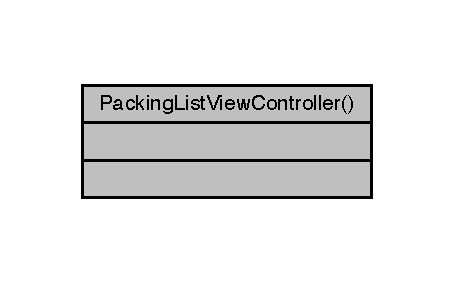
\includegraphics[width=218pt]{category_packing_list_view_controller_07_08__coll__graph}
\end{center}
\end{figure}
\subsection*{Properties}
\begin{DoxyCompactItemize}
\item 
\hypertarget{category_packing_list_view_controller_07_08_aa490f06ed76cbd8f0d6094aa8df72a6b}{N\-S\-Integer {\bfseries selected\-Index}}\label{category_packing_list_view_controller_07_08_aa490f06ed76cbd8f0d6094aa8df72a6b}

\end{DoxyCompactItemize}


The documentation for this category was generated from the following file\-:\begin{DoxyCompactItemize}
\item 
Pack\-Manager/Packing\-List\-View\-Controller.\-m\end{DoxyCompactItemize}

\hypertarget{interface_pack_manager_tests}{\section{Pack\-Manager\-Tests Class Reference}
\label{interface_pack_manager_tests}\index{Pack\-Manager\-Tests@{Pack\-Manager\-Tests}}
}


Inheritance diagram for Pack\-Manager\-Tests\-:\nopagebreak
\begin{figure}[H]
\begin{center}
\leavevmode
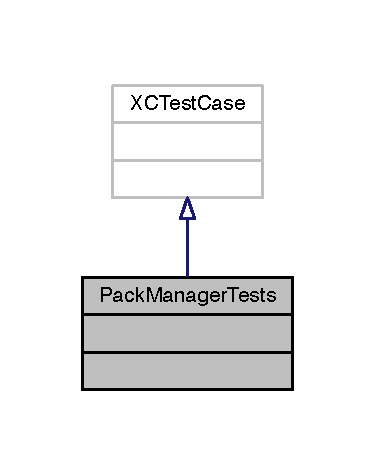
\includegraphics[width=180pt]{interface_pack_manager_tests__inherit__graph}
\end{center}
\end{figure}


Collaboration diagram for Pack\-Manager\-Tests\-:\nopagebreak
\begin{figure}[H]
\begin{center}
\leavevmode
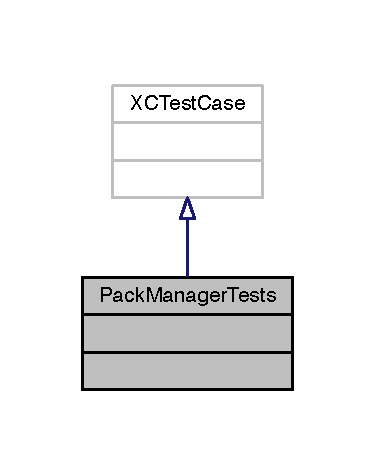
\includegraphics[width=180pt]{interface_pack_manager_tests__coll__graph}
\end{center}
\end{figure}


The documentation for this class was generated from the following file\-:\begin{DoxyCompactItemize}
\item 
Pack\-Manager\-Tests/Pack\-Manager\-Tests.\-m\end{DoxyCompactItemize}

\hypertarget{interface_profile_view_controller}{\section{Profile\-View\-Controller Class Reference}
\label{interface_profile_view_controller}\index{Profile\-View\-Controller@{Profile\-View\-Controller}}
}


Inheritance diagram for Profile\-View\-Controller\-:\nopagebreak
\begin{figure}[H]
\begin{center}
\leavevmode
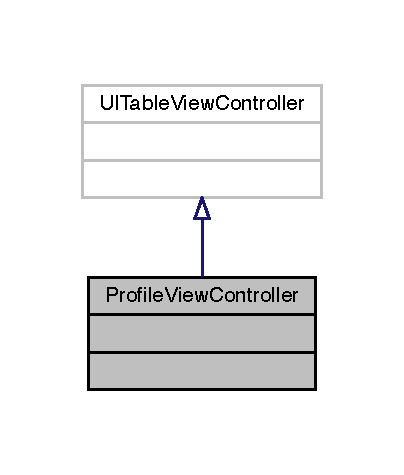
\includegraphics[width=194pt]{interface_profile_view_controller__inherit__graph}
\end{center}
\end{figure}


Collaboration diagram for Profile\-View\-Controller\-:\nopagebreak
\begin{figure}[H]
\begin{center}
\leavevmode
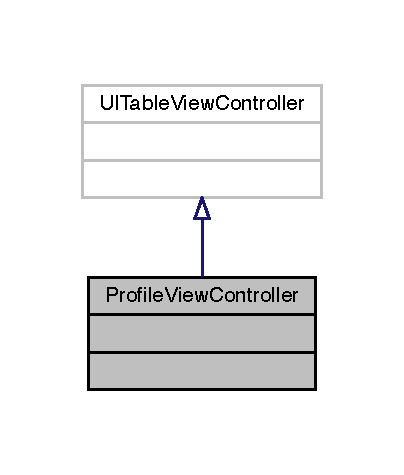
\includegraphics[width=194pt]{interface_profile_view_controller__coll__graph}
\end{center}
\end{figure}


The documentation for this class was generated from the following file\-:\begin{DoxyCompactItemize}
\item 
Pack\-Manager/Profile\-View\-Controller.\-h\end{DoxyCompactItemize}

\hypertarget{category_profile_view_controller_07_08}{\section{Profile\-View\-Controller() Category Reference}
\label{category_profile_view_controller_07_08}\index{Profile\-View\-Controller()@{Profile\-View\-Controller()}}
}


Collaboration diagram for Profile\-View\-Controller()\-:\nopagebreak
\begin{figure}[H]
\begin{center}
\leavevmode
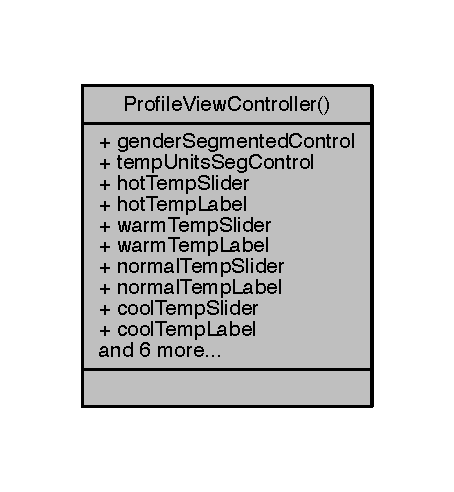
\includegraphics[width=218pt]{category_profile_view_controller_07_08__coll__graph}
\end{center}
\end{figure}
\subsection*{Properties}
\begin{DoxyCompactItemize}
\item 
\hypertarget{category_profile_view_controller_07_08_afade1346814bb19908adb2a80592b588}{I\-B\-Outlet U\-I\-Segmented\-Control $\ast$ {\bfseries gender\-Segmented\-Control}}\label{category_profile_view_controller_07_08_afade1346814bb19908adb2a80592b588}

\item 
\hypertarget{category_profile_view_controller_07_08_a1f6259c4ee51c1c87b1e80b68fa08df6}{I\-B\-Outlet U\-I\-Segmented\-Control $\ast$ {\bfseries temp\-Units\-Seg\-Control}}\label{category_profile_view_controller_07_08_a1f6259c4ee51c1c87b1e80b68fa08df6}

\item 
\hypertarget{category_profile_view_controller_07_08_a62fb51366cd4d0179175cf35537ef632}{I\-B\-Outlet U\-I\-Slider $\ast$ {\bfseries hot\-Temp\-Slider}}\label{category_profile_view_controller_07_08_a62fb51366cd4d0179175cf35537ef632}

\item 
\hypertarget{category_profile_view_controller_07_08_a497d03279c625051a88ce9b56687f045}{I\-B\-Outlet U\-I\-Label $\ast$ {\bfseries hot\-Temp\-Label}}\label{category_profile_view_controller_07_08_a497d03279c625051a88ce9b56687f045}

\item 
\hypertarget{category_profile_view_controller_07_08_aa3d25b97cba911a3af38912b1f059f7b}{I\-B\-Outlet U\-I\-Slider $\ast$ {\bfseries warm\-Temp\-Slider}}\label{category_profile_view_controller_07_08_aa3d25b97cba911a3af38912b1f059f7b}

\item 
\hypertarget{category_profile_view_controller_07_08_ac994f98d8cdabb165059be14863b4e4b}{I\-B\-Outlet U\-I\-Label $\ast$ {\bfseries warm\-Temp\-Label}}\label{category_profile_view_controller_07_08_ac994f98d8cdabb165059be14863b4e4b}

\item 
\hypertarget{category_profile_view_controller_07_08_a22464da0e5a89b0440f9b4d1b8df702c}{I\-B\-Outlet U\-I\-Slider $\ast$ {\bfseries normal\-Temp\-Slider}}\label{category_profile_view_controller_07_08_a22464da0e5a89b0440f9b4d1b8df702c}

\item 
\hypertarget{category_profile_view_controller_07_08_a83aac2bb65b452dda4c652f8ca2f43f1}{I\-B\-Outlet U\-I\-Label $\ast$ {\bfseries normal\-Temp\-Label}}\label{category_profile_view_controller_07_08_a83aac2bb65b452dda4c652f8ca2f43f1}

\item 
\hypertarget{category_profile_view_controller_07_08_a8a9ce9eaac3d75ce587e689fbe598df2}{I\-B\-Outlet U\-I\-Slider $\ast$ {\bfseries cool\-Temp\-Slider}}\label{category_profile_view_controller_07_08_a8a9ce9eaac3d75ce587e689fbe598df2}

\item 
\hypertarget{category_profile_view_controller_07_08_aee8c55e0c0ca0c5d1962b88bc1c6c1c5}{I\-B\-Outlet U\-I\-Label $\ast$ {\bfseries cool\-Temp\-Label}}\label{category_profile_view_controller_07_08_aee8c55e0c0ca0c5d1962b88bc1c6c1c5}

\item 
\hypertarget{category_profile_view_controller_07_08_a9f7c13a860eb2ea38a1c0064a126c312}{I\-B\-Outlet U\-I\-Slider $\ast$ {\bfseries cold\-Temp\-Slider}}\label{category_profile_view_controller_07_08_a9f7c13a860eb2ea38a1c0064a126c312}

\item 
\hypertarget{category_profile_view_controller_07_08_afe8b73929d3ae3bfd3b98eda41ce443f}{I\-B\-Outlet U\-I\-Label $\ast$ {\bfseries cold\-Temp\-Label}}\label{category_profile_view_controller_07_08_afe8b73929d3ae3bfd3b98eda41ce443f}

\item 
\hypertarget{category_profile_view_controller_07_08_a6bd271b6f0cd9c4a2f18bec7eb09063e}{I\-B\-Outlet U\-I\-Switch $\ast$ {\bfseries swimming\-Preference\-Switch}}\label{category_profile_view_controller_07_08_a6bd271b6f0cd9c4a2f18bec7eb09063e}

\item 
\hypertarget{category_profile_view_controller_07_08_aae60ad5fd771b0aae83227268ddf2546}{I\-B\-Outlet U\-I\-Switch $\ast$ {\bfseries rewear\-Jeans\-Preference\-Switch}}\label{category_profile_view_controller_07_08_aae60ad5fd771b0aae83227268ddf2546}

\item 
\hypertarget{category_profile_view_controller_07_08_ac65a8528c99524566c2002530cb60fcd}{I\-B\-Outlet U\-I\-Switch $\ast$ {\bfseries formal\-Preference\-Switch}}\label{category_profile_view_controller_07_08_ac65a8528c99524566c2002530cb60fcd}

\item 
\hypertarget{category_profile_view_controller_07_08_a2038df29da26d89e9b2f81b3c4d2f982}{I\-B\-Outlet U\-I\-Switch $\ast$ {\bfseries access\-To\-Laundry\-Preference\-Switch}}\label{category_profile_view_controller_07_08_a2038df29da26d89e9b2f81b3c4d2f982}

\end{DoxyCompactItemize}


The documentation for this category was generated from the following file\-:\begin{DoxyCompactItemize}
\item 
Pack\-Manager/Profile\-View\-Controller.\-m\end{DoxyCompactItemize}

\hypertarget{interface_trip}{\section{Trip Class Reference}
\label{interface_trip}\index{Trip@{Trip}}
}


{\ttfamily \#import $<$Trip.\-h$>$}



Inheritance diagram for Trip\-:\nopagebreak
\begin{figure}[H]
\begin{center}
\leavevmode
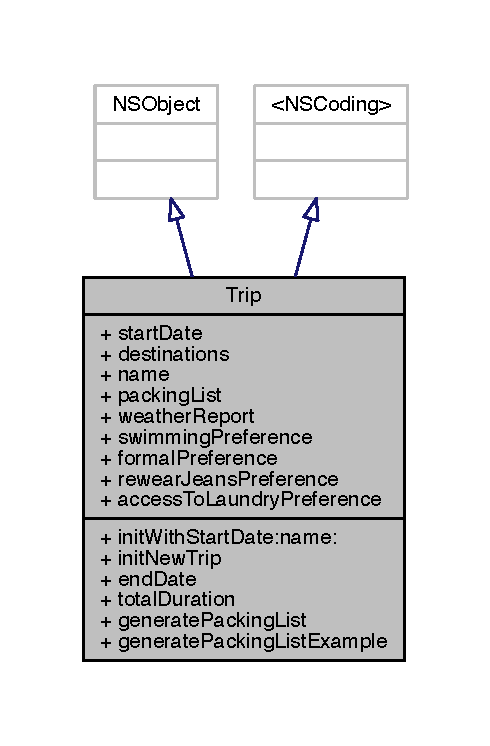
\includegraphics[width=235pt]{interface_trip__inherit__graph}
\end{center}
\end{figure}


Collaboration diagram for Trip\-:\nopagebreak
\begin{figure}[H]
\begin{center}
\leavevmode
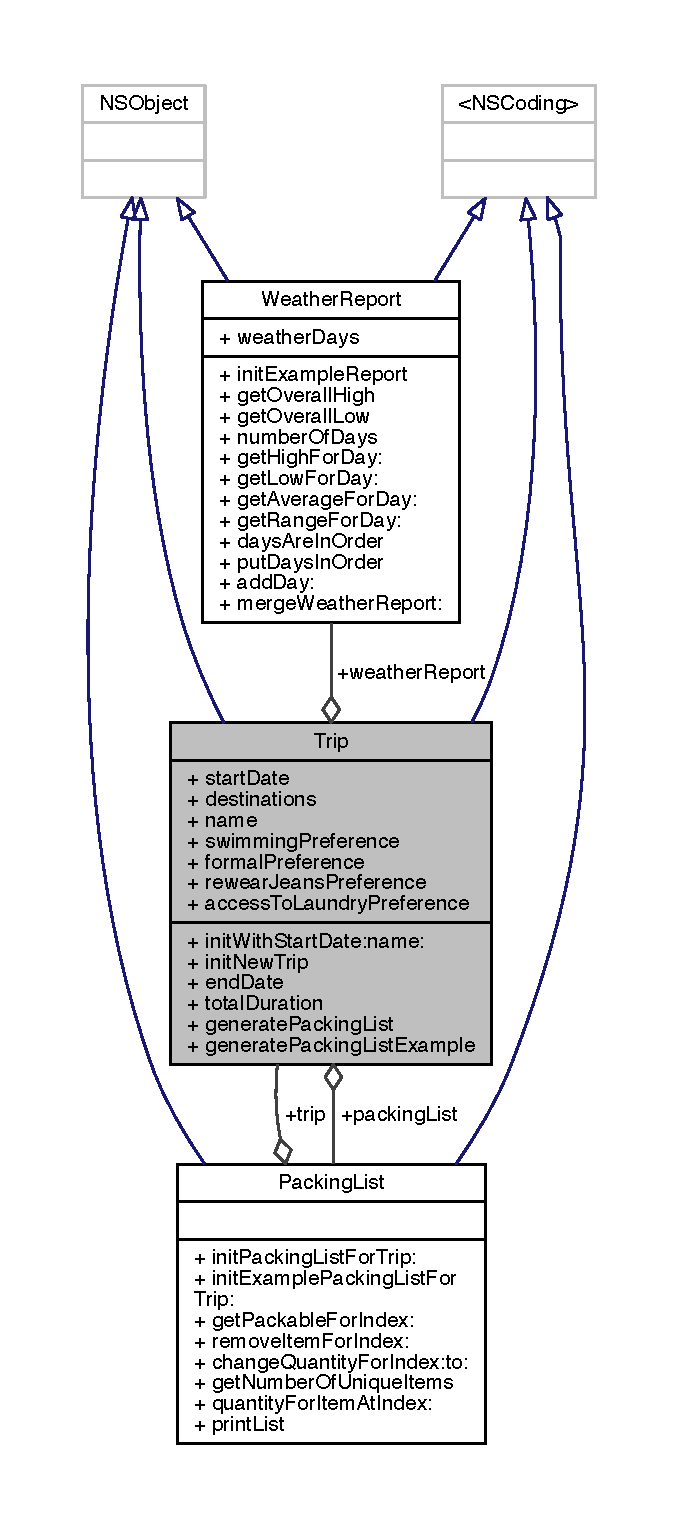
\includegraphics[width=350pt]{interface_trip__coll__graph}
\end{center}
\end{figure}
\subsection*{Instance Methods}
\begin{DoxyCompactItemize}
\item 
(instancetype) -\/ \hyperlink{interface_trip_aca341893b609059158a3c2809d5fd157}{init\-With\-Start\-Date\-:name\-:}
\item 
(instancetype) -\/ \hyperlink{interface_trip_ab712f4d482a0a2818038069998aea9aa}{init\-New\-Trip}
\item 
(N\-S\-Date $\ast$) -\/ \hyperlink{interface_trip_af45eceb7475c6e48bf48641deb44baf4}{end\-Date}
\item 
(N\-S\-Integer) -\/ \hyperlink{interface_trip_a7d4e8ffcab800bda331f75625eb2c6d3}{total\-Duration}
\item 
(B\-O\-O\-L) -\/ \hyperlink{interface_trip_a90808fe2b7874349bf0a5fc5a09acf3e}{generate\-Packing\-List}
\item 
(B\-O\-O\-L) -\/ \hyperlink{interface_trip_a078c437bbefc9fe136a03093fd549b10}{generate\-Packing\-List\-Example}
\end{DoxyCompactItemize}
\subsection*{Properties}
\begin{DoxyCompactItemize}
\item 
N\-S\-Date $\ast$ \hyperlink{interface_trip_aa73721dd452a5a0c94841aa155761d67}{start\-Date}
\item 
N\-S\-Mutable\-Array $\ast$ \hyperlink{interface_trip_a396ca8de2ed1b20c1255cbb5e9b524ed}{destinations}
\item 
N\-S\-String $\ast$ \hyperlink{interface_trip_a66e63287102687fe25366d61889fe8e1}{name}
\item 
\hyperlink{interface_packing_list}{Packing\-List} $\ast$ \hyperlink{interface_trip_a985205885a33d59e7e8b899cab47f2d0}{packing\-List}
\item 
\hyperlink{interface_weather_report}{Weather\-Report} $\ast$ \hyperlink{interface_trip_a50df03c3a57389928c170792a63aa67f}{weather\-Report}
\item 
B\-O\-O\-L \hyperlink{interface_trip_a3f7f9fac616d0861b0229a31aa485f39}{swimming\-Preference}
\item 
B\-O\-O\-L \hyperlink{interface_trip_a4ea48dfbac9dff7d387617f1113c3d08}{formal\-Preference}
\item 
B\-O\-O\-L \hyperlink{interface_trip_a0a0bd7f81cb9866501819178b9167fad}{rewear\-Jeans\-Preference}
\item 
B\-O\-O\-L \hyperlink{interface_trip_a5807a192e5170272e808780c5e74ca5a}{access\-To\-Laundry\-Preference}
\end{DoxyCompactItemize}


\subsection{Detailed Description}
A class to represent a trip

\hyperlink{interface_trip}{Trip} object that contains all necessary information for a trip, including the packing lists and weather information. This data structure will be passed around frequently for populating the core U\-I of many screens. 

\subsection{Method Documentation}
\hypertarget{interface_trip_af45eceb7475c6e48bf48641deb44baf4}{\index{Trip@{Trip}!end\-Date@{end\-Date}}
\index{end\-Date@{end\-Date}!Trip@{Trip}}
\subsubsection[{end\-Date}]{\setlength{\rightskip}{0pt plus 5cm}-\/ (N\-S\-Date $\ast$) end\-Date 
\begin{DoxyParamCaption}
{}
\end{DoxyParamCaption}
}}\label{interface_trip_af45eceb7475c6e48bf48641deb44baf4}
Helper Function\-: Returns end date of trip \begin{DoxyReturn}{Returns}
date of trip's end 
\end{DoxyReturn}
\hypertarget{interface_trip_a90808fe2b7874349bf0a5fc5a09acf3e}{\index{Trip@{Trip}!generate\-Packing\-List@{generate\-Packing\-List}}
\index{generate\-Packing\-List@{generate\-Packing\-List}!Trip@{Trip}}
\subsubsection[{generate\-Packing\-List}]{\setlength{\rightskip}{0pt plus 5cm}-\/ (B\-O\-O\-L) generate\-Packing\-List 
\begin{DoxyParamCaption}
{}
\end{DoxyParamCaption}
}}\label{interface_trip_a90808fe2b7874349bf0a5fc5a09acf3e}
This is the big one. Returns true if everything went O\-K and the packing list is created, false otherwise.

Examples for why it might return false\-:
\begin{DoxyItemize}
\item invalid destination
\item invalid or N\-U\-L\-L weather report
\item start date / duration is N\-U\-L\-L \begin{DoxyReturn}{Returns}
T\-R\-U\-E if everything went ok, otherwise returns F\-A\-L\-S\-E 
\end{DoxyReturn}

\end{DoxyItemize}\hypertarget{interface_trip_a078c437bbefc9fe136a03093fd549b10}{\index{Trip@{Trip}!generate\-Packing\-List\-Example@{generate\-Packing\-List\-Example}}
\index{generate\-Packing\-List\-Example@{generate\-Packing\-List\-Example}!Trip@{Trip}}
\subsubsection[{generate\-Packing\-List\-Example}]{\setlength{\rightskip}{0pt plus 5cm}-\/ (B\-O\-O\-L) generate\-Packing\-List\-Example 
\begin{DoxyParamCaption}
{}
\end{DoxyParamCaption}
}}\label{interface_trip_a078c437bbefc9fe136a03093fd549b10}
Creates a generic packing list for demo purposes only. \begin{DoxyReturn}{Returns}
T\-R\-U\-E always 
\end{DoxyReturn}
\hypertarget{interface_trip_ab712f4d482a0a2818038069998aea9aa}{\index{Trip@{Trip}!init\-New\-Trip@{init\-New\-Trip}}
\index{init\-New\-Trip@{init\-New\-Trip}!Trip@{Trip}}
\subsubsection[{init\-New\-Trip}]{\setlength{\rightskip}{0pt plus 5cm}-\/ (instancetype) init\-New\-Trip 
\begin{DoxyParamCaption}
{}
\end{DoxyParamCaption}
}}\label{interface_trip_ab712f4d482a0a2818038069998aea9aa}
Initialize a new \hyperlink{interface_trip}{Trip} object \begin{DoxyReturn}{Returns}
a newly initialized object 
\end{DoxyReturn}
\hypertarget{interface_trip_aca341893b609059158a3c2809d5fd157}{\index{Trip@{Trip}!init\-With\-Start\-Date\-:name\-:@{init\-With\-Start\-Date\-:name\-:}}
\index{init\-With\-Start\-Date\-:name\-:@{init\-With\-Start\-Date\-:name\-:}!Trip@{Trip}}
\subsubsection[{init\-With\-Start\-Date\-:name\-:}]{\setlength{\rightskip}{0pt plus 5cm}-\/ (instancetype) init\-With\-Start\-Date\-: 
\begin{DoxyParamCaption}
\item[{(N\-S\-Date $\ast$)}]{start}
\item[{name:(N\-S\-String $\ast$)}]{name}
\end{DoxyParamCaption}
}}\label{interface_trip_aca341893b609059158a3c2809d5fd157}
Initialize a new \hyperlink{interface_trip}{Trip} object 
\begin{DoxyParams}{Parameters}
{\em start} & The trip start date \\
\hline
{\em name} & The trip name \\
\hline
\end{DoxyParams}
\begin{DoxyReturn}{Returns}
a newly initialized object
\end{DoxyReturn}
Creates new trip with given parameters. 
\begin{DoxyParams}{Parameters}
{\em start} & start date of the trip \\
\hline
{\em name} & the name of the trip \\
\hline
\end{DoxyParams}
\hypertarget{interface_trip_a7d4e8ffcab800bda331f75625eb2c6d3}{\index{Trip@{Trip}!total\-Duration@{total\-Duration}}
\index{total\-Duration@{total\-Duration}!Trip@{Trip}}
\subsubsection[{total\-Duration}]{\setlength{\rightskip}{0pt plus 5cm}-\/ (N\-S\-Integer) total\-Duration 
\begin{DoxyParamCaption}
{}
\end{DoxyParamCaption}
}}\label{interface_trip_a7d4e8ffcab800bda331f75625eb2c6d3}
Returns the total number of days for the trip. 

\subsection{Property Documentation}
\hypertarget{interface_trip_a5807a192e5170272e808780c5e74ca5a}{\index{Trip@{Trip}!access\-To\-Laundry\-Preference@{access\-To\-Laundry\-Preference}}
\index{access\-To\-Laundry\-Preference@{access\-To\-Laundry\-Preference}!Trip@{Trip}}
\subsubsection[{access\-To\-Laundry\-Preference}]{\setlength{\rightskip}{0pt plus 5cm}-\/ (B\-O\-O\-L) access\-To\-Laundry\-Preference\hspace{0.3cm}{\ttfamily [read]}, {\ttfamily [write]}, {\ttfamily [atomic]}}}\label{interface_trip_a5807a192e5170272e808780c5e74ca5a}
Bool\-: Will the user be able to do laundry on the trip \hypertarget{interface_trip_a396ca8de2ed1b20c1255cbb5e9b524ed}{\index{Trip@{Trip}!destinations@{destinations}}
\index{destinations@{destinations}!Trip@{Trip}}
\subsubsection[{destinations}]{\setlength{\rightskip}{0pt plus 5cm}-\/ (N\-S\-Mutable\-Array$\ast$) destinations\hspace{0.3cm}{\ttfamily [read]}, {\ttfamily [write]}, {\ttfamily [nonatomic]}, {\ttfamily [strong]}}}\label{interface_trip_a396ca8de2ed1b20c1255cbb5e9b524ed}
The trip's destinations \hypertarget{interface_trip_a4ea48dfbac9dff7d387617f1113c3d08}{\index{Trip@{Trip}!formal\-Preference@{formal\-Preference}}
\index{formal\-Preference@{formal\-Preference}!Trip@{Trip}}
\subsubsection[{formal\-Preference}]{\setlength{\rightskip}{0pt plus 5cm}-\/ (B\-O\-O\-L) formal\-Preference\hspace{0.3cm}{\ttfamily [read]}, {\ttfamily [write]}, {\ttfamily [atomic]}}}\label{interface_trip_a4ea48dfbac9dff7d387617f1113c3d08}
Bool\-: Will the user require formal clothing \hypertarget{interface_trip_a66e63287102687fe25366d61889fe8e1}{\index{Trip@{Trip}!name@{name}}
\index{name@{name}!Trip@{Trip}}
\subsubsection[{name}]{\setlength{\rightskip}{0pt plus 5cm}-\/ (N\-S\-String$\ast$) name\hspace{0.3cm}{\ttfamily [read]}, {\ttfamily [write]}, {\ttfamily [nonatomic]}, {\ttfamily [strong]}}}\label{interface_trip_a66e63287102687fe25366d61889fe8e1}
The name of the trip \hypertarget{interface_trip_a985205885a33d59e7e8b899cab47f2d0}{\index{Trip@{Trip}!packing\-List@{packing\-List}}
\index{packing\-List@{packing\-List}!Trip@{Trip}}
\subsubsection[{packing\-List}]{\setlength{\rightskip}{0pt plus 5cm}-\/ ({\bf Packing\-List}$\ast$) packing\-List\hspace{0.3cm}{\ttfamily [read]}, {\ttfamily [write]}, {\ttfamily [nonatomic]}, {\ttfamily [strong]}}}\label{interface_trip_a985205885a33d59e7e8b899cab47f2d0}
The packing list for the trip \hypertarget{interface_trip_a0a0bd7f81cb9866501819178b9167fad}{\index{Trip@{Trip}!rewear\-Jeans\-Preference@{rewear\-Jeans\-Preference}}
\index{rewear\-Jeans\-Preference@{rewear\-Jeans\-Preference}!Trip@{Trip}}
\subsubsection[{rewear\-Jeans\-Preference}]{\setlength{\rightskip}{0pt plus 5cm}-\/ (B\-O\-O\-L) rewear\-Jeans\-Preference\hspace{0.3cm}{\ttfamily [read]}, {\ttfamily [write]}, {\ttfamily [atomic]}}}\label{interface_trip_a0a0bd7f81cb9866501819178b9167fad}
Bool\-: Will the user rewear unwashed jeans \hypertarget{interface_trip_aa73721dd452a5a0c94841aa155761d67}{\index{Trip@{Trip}!start\-Date@{start\-Date}}
\index{start\-Date@{start\-Date}!Trip@{Trip}}
\subsubsection[{start\-Date}]{\setlength{\rightskip}{0pt plus 5cm}-\/ (N\-S\-Date$\ast$) start\-Date\hspace{0.3cm}{\ttfamily [read]}, {\ttfamily [write]}, {\ttfamily [nonatomic]}, {\ttfamily [strong]}}}\label{interface_trip_aa73721dd452a5a0c94841aa155761d67}
The start date of the trip \hypertarget{interface_trip_a3f7f9fac616d0861b0229a31aa485f39}{\index{Trip@{Trip}!swimming\-Preference@{swimming\-Preference}}
\index{swimming\-Preference@{swimming\-Preference}!Trip@{Trip}}
\subsubsection[{swimming\-Preference}]{\setlength{\rightskip}{0pt plus 5cm}-\/ (B\-O\-O\-L) swimming\-Preference\hspace{0.3cm}{\ttfamily [read]}, {\ttfamily [write]}, {\ttfamily [atomic]}}}\label{interface_trip_a3f7f9fac616d0861b0229a31aa485f39}
Bool\-: Will the user be swimming on the trip \hypertarget{interface_trip_a50df03c3a57389928c170792a63aa67f}{\index{Trip@{Trip}!weather\-Report@{weather\-Report}}
\index{weather\-Report@{weather\-Report}!Trip@{Trip}}
\subsubsection[{weather\-Report}]{\setlength{\rightskip}{0pt plus 5cm}-\/ ({\bf Weather\-Report}$\ast$) weather\-Report\hspace{0.3cm}{\ttfamily [read]}, {\ttfamily [write]}, {\ttfamily [nonatomic]}, {\ttfamily [strong]}}}\label{interface_trip_a50df03c3a57389928c170792a63aa67f}
The weather report for the trip 

The documentation for this class was generated from the following files\-:\begin{DoxyCompactItemize}
\item 
Pack\-Manager/Trip.\-h\item 
Pack\-Manager/Trip.\-m\end{DoxyCompactItemize}

\hypertarget{interface_trips_data}{\section{Trips\-Data Class Reference}
\label{interface_trips_data}\index{Trips\-Data@{Trips\-Data}}
}


Inheritance diagram for Trips\-Data\-:\nopagebreak
\begin{figure}[H]
\begin{center}
\leavevmode
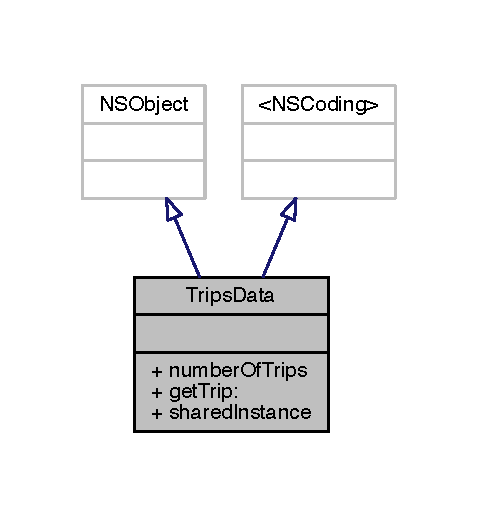
\includegraphics[width=229pt]{interface_trips_data__inherit__graph}
\end{center}
\end{figure}


Collaboration diagram for Trips\-Data\-:\nopagebreak
\begin{figure}[H]
\begin{center}
\leavevmode
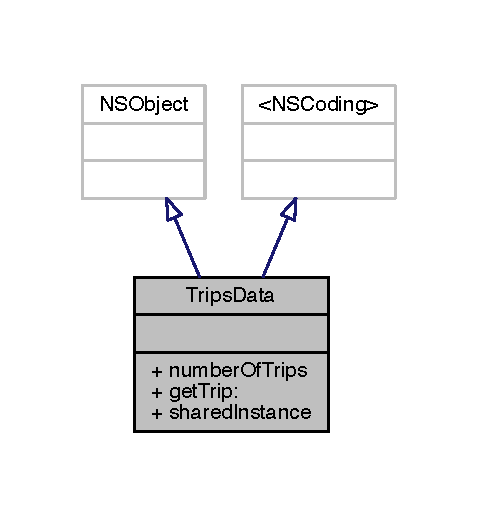
\includegraphics[width=229pt]{interface_trips_data__coll__graph}
\end{center}
\end{figure}
\subsection*{Instance Methods}
\begin{DoxyCompactItemize}
\item 
\hypertarget{interface_trips_data_aaad503ab67656b4e43ad6227fba6fc59}{(N\-S\-Integer) -\/ {\bfseries number\-Of\-Trips}}\label{interface_trips_data_aaad503ab67656b4e43ad6227fba6fc59}

\item 
\hypertarget{interface_trips_data_a433034d39dff68774a32958007ad5ff1}{(\hyperlink{interface_trip}{Trip} $\ast$) -\/ {\bfseries get\-Trip\-:}}\label{interface_trips_data_a433034d39dff68774a32958007ad5ff1}

\end{DoxyCompactItemize}
\subsection*{Class Methods}
\begin{DoxyCompactItemize}
\item 
\hypertarget{interface_trips_data_ac78fc79e8ebd10722f0b9f06df78eb27}{(instancetype) + {\bfseries shared\-Instance}}\label{interface_trips_data_ac78fc79e8ebd10722f0b9f06df78eb27}

\end{DoxyCompactItemize}


The documentation for this class was generated from the following files\-:\begin{DoxyCompactItemize}
\item 
Pack\-Manager/Trips\-Data.\-h\item 
Pack\-Manager/Trips\-Data.\-m\end{DoxyCompactItemize}

\hypertarget{category_trips_data_07_08}{\section{Trips\-Data() Category Reference}
\label{category_trips_data_07_08}\index{Trips\-Data()@{Trips\-Data()}}
}


Collaboration diagram for Trips\-Data()\-:\nopagebreak
\begin{figure}[H]
\begin{center}
\leavevmode
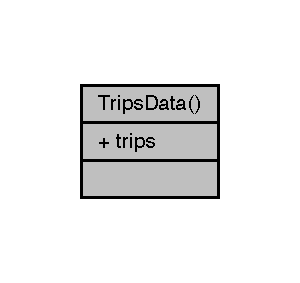
\includegraphics[width=144pt]{category_trips_data_07_08__coll__graph}
\end{center}
\end{figure}
\subsection*{Properties}
\begin{DoxyCompactItemize}
\item 
\hypertarget{category_trips_data_07_08_ad32a793f3e7c3eaa529ea0c57fef9b42}{N\-S\-Mutable\-Array $\ast$ {\bfseries trips}}\label{category_trips_data_07_08_ad32a793f3e7c3eaa529ea0c57fef9b42}

\end{DoxyCompactItemize}


The documentation for this category was generated from the following file\-:\begin{DoxyCompactItemize}
\item 
Pack\-Manager/Trips\-Data.\-m\end{DoxyCompactItemize}

\hypertarget{interface_trip_settings_view_controller}{\section{Trip\-Settings\-View\-Controller Class Reference}
\label{interface_trip_settings_view_controller}\index{Trip\-Settings\-View\-Controller@{Trip\-Settings\-View\-Controller}}
}


Inheritance diagram for Trip\-Settings\-View\-Controller\-:\nopagebreak
\begin{figure}[H]
\begin{center}
\leavevmode
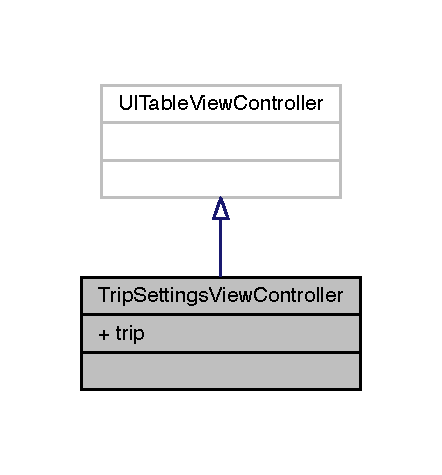
\includegraphics[width=212pt]{interface_trip_settings_view_controller__inherit__graph}
\end{center}
\end{figure}


Collaboration diagram for Trip\-Settings\-View\-Controller\-:
\nopagebreak
\begin{figure}[H]
\begin{center}
\leavevmode
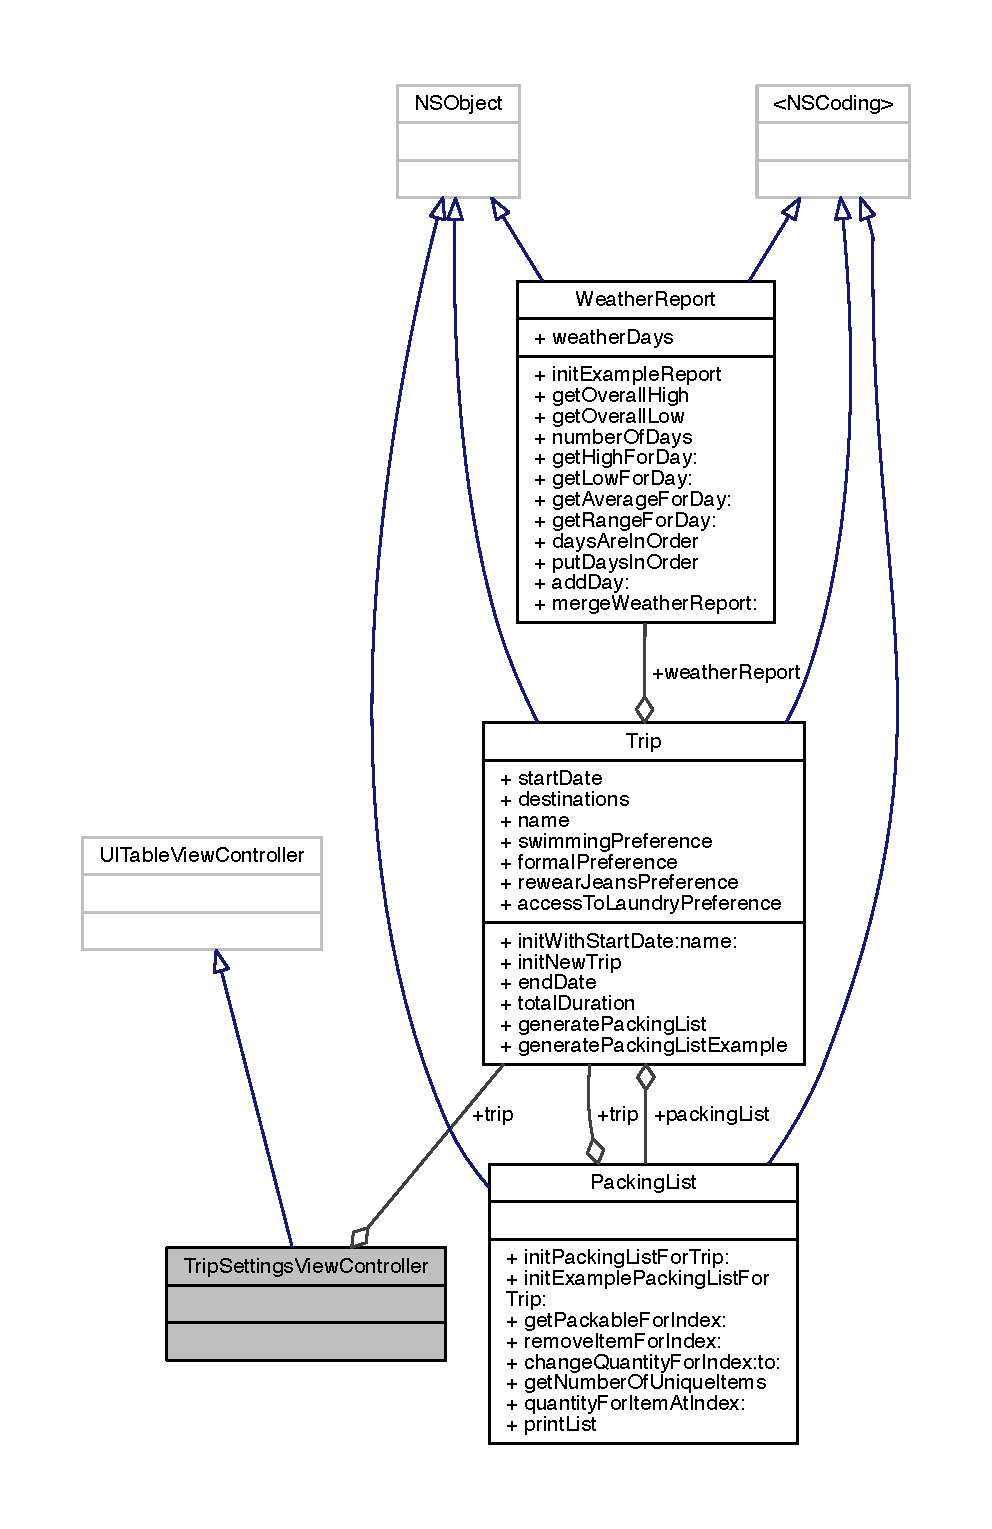
\includegraphics[width=350pt]{interface_trip_settings_view_controller__coll__graph}
\end{center}
\end{figure}
\subsection*{Properties}
\begin{DoxyCompactItemize}
\item 
\hypertarget{interface_trip_settings_view_controller_a2faba5a7d0de3f72b88a18801c2b0be4}{\hyperlink{interface_trip}{Trip} $\ast$ {\bfseries trip}}\label{interface_trip_settings_view_controller_a2faba5a7d0de3f72b88a18801c2b0be4}

\end{DoxyCompactItemize}


The documentation for this class was generated from the following file\-:\begin{DoxyCompactItemize}
\item 
Pack\-Manager/Trip\-Settings\-View\-Controller.\-h\end{DoxyCompactItemize}

\hypertarget{category_trip_settings_view_controller_07_08}{\section{Trip\-Settings\-View\-Controller() Category Reference}
\label{category_trip_settings_view_controller_07_08}\index{Trip\-Settings\-View\-Controller()@{Trip\-Settings\-View\-Controller()}}
}


Collaboration diagram for Trip\-Settings\-View\-Controller()\-:\nopagebreak
\begin{figure}[H]
\begin{center}
\leavevmode
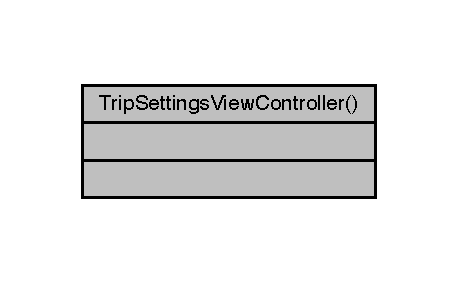
\includegraphics[width=220pt]{category_trip_settings_view_controller_07_08__coll__graph}
\end{center}
\end{figure}


The documentation for this category was generated from the following file\-:\begin{DoxyCompactItemize}
\item 
Pack\-Manager/Trip\-Settings\-View\-Controller.\-m\end{DoxyCompactItemize}

\hypertarget{interface_trips_view_controller}{\section{Trips\-View\-Controller Class Reference}
\label{interface_trips_view_controller}\index{Trips\-View\-Controller@{Trips\-View\-Controller}}
}


Inheritance diagram for Trips\-View\-Controller\-:\nopagebreak
\begin{figure}[H]
\begin{center}
\leavevmode
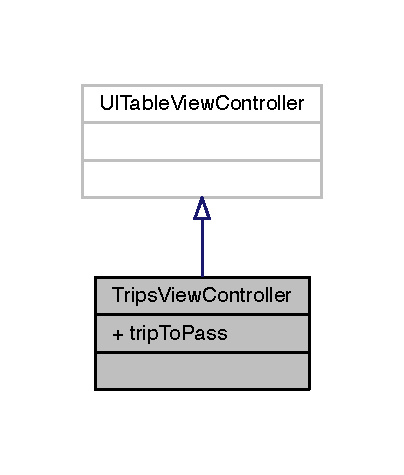
\includegraphics[width=194pt]{interface_trips_view_controller__inherit__graph}
\end{center}
\end{figure}


Collaboration diagram for Trips\-View\-Controller\-:
\nopagebreak
\begin{figure}[H]
\begin{center}
\leavevmode
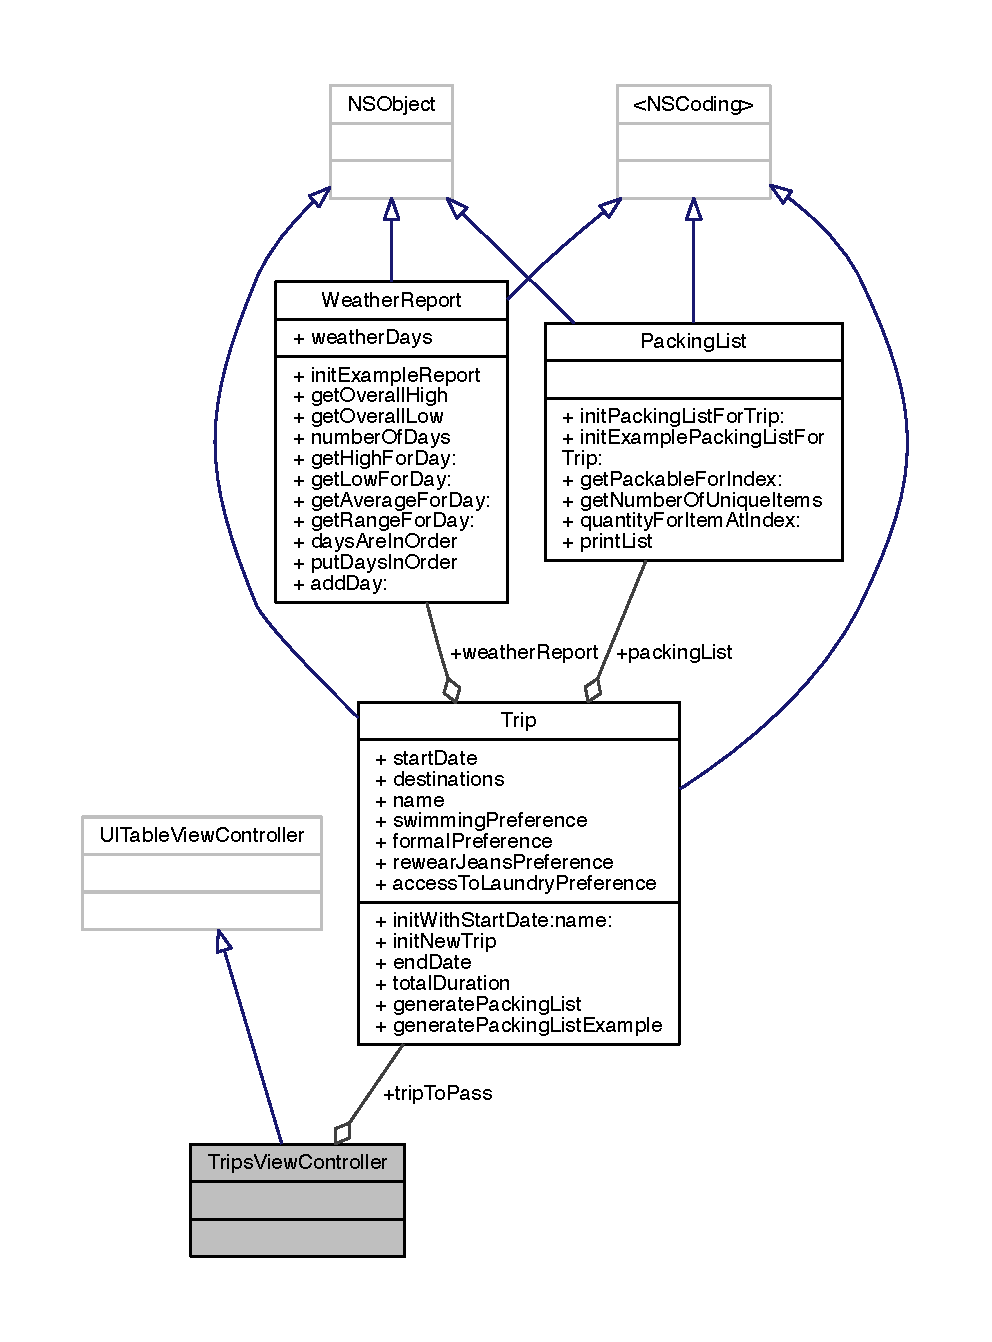
\includegraphics[width=350pt]{interface_trips_view_controller__coll__graph}
\end{center}
\end{figure}
\subsection*{Properties}
\begin{DoxyCompactItemize}
\item 
\hypertarget{interface_trips_view_controller_aefdf3056f500f9c958e6d42ae444bb31}{\hyperlink{interface_trip}{Trip} $\ast$ {\bfseries trip\-To\-Pass}}\label{interface_trips_view_controller_aefdf3056f500f9c958e6d42ae444bb31}

\end{DoxyCompactItemize}


The documentation for this class was generated from the following file\-:\begin{DoxyCompactItemize}
\item 
Pack\-Manager/Trips\-View\-Controller.\-h\end{DoxyCompactItemize}

\hypertarget{category_trips_view_controller_07_08}{\section{Trips\-View\-Controller() Category Reference}
\label{category_trips_view_controller_07_08}\index{Trips\-View\-Controller()@{Trips\-View\-Controller()}}
}


Collaboration diagram for Trips\-View\-Controller()\-:\nopagebreak
\begin{figure}[H]
\begin{center}
\leavevmode
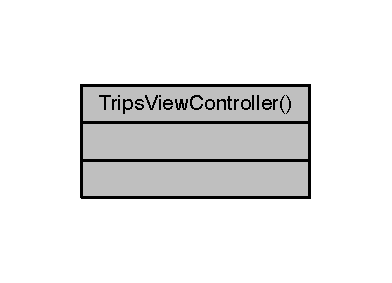
\includegraphics[width=188pt]{category_trips_view_controller_07_08__coll__graph}
\end{center}
\end{figure}


The documentation for this category was generated from the following file\-:\begin{DoxyCompactItemize}
\item 
Pack\-Manager/Trips\-View\-Controller.\-m\end{DoxyCompactItemize}

\hypertarget{interface_weather_a_p_i}{\section{Weather\-A\-P\-I Class Reference}
\label{interface_weather_a_p_i}\index{Weather\-A\-P\-I@{Weather\-A\-P\-I}}
}


Inheritance diagram for Weather\-A\-P\-I\-:\nopagebreak
\begin{figure}[H]
\begin{center}
\leavevmode
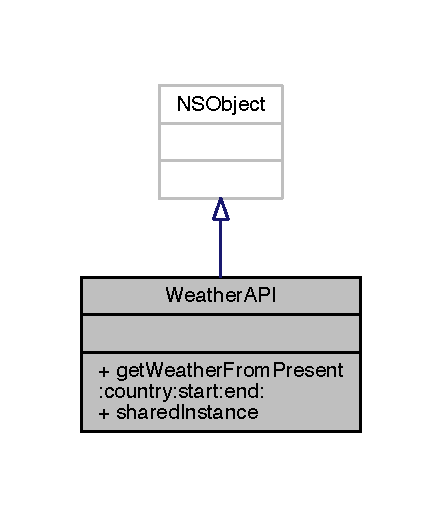
\includegraphics[width=230pt]{interface_weather_a_p_i__inherit__graph}
\end{center}
\end{figure}


Collaboration diagram for Weather\-A\-P\-I\-:\nopagebreak
\begin{figure}[H]
\begin{center}
\leavevmode
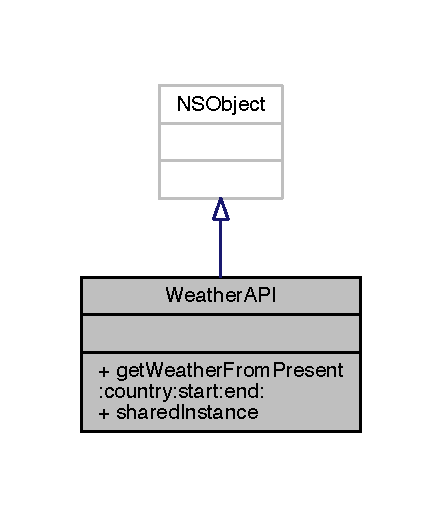
\includegraphics[width=230pt]{interface_weather_a_p_i__coll__graph}
\end{center}
\end{figure}
\subsection*{Instance Methods}
\begin{DoxyCompactItemize}
\item 
(\hyperlink{interface_weather_report}{Weather\-Report} $\ast$) -\/ \hyperlink{interface_weather_a_p_i_aec65367ed89cc10d855a561a01819a61}{get\-Weather\-Report\-:start\-:end\-:}
\item 
(\hyperlink{interface_weather_report}{Weather\-Report} $\ast$) -\/ \hyperlink{interface_weather_a_p_i_a923043c755894633e58b7d8dbd164a30}{get\-Weather\-Report\-:start\-:end\-:lat\-:lon\-:}
\item 
(N\-S\-Mutable\-Array $\ast$) -\/ \hyperlink{interface_weather_a_p_i_aa3c918e845c1788e0802e67a1a7fd0d7}{get\-Weather\-From\-Present\-:lng\-:start\-:end\-:}
\item 
(N\-S\-Mutable\-Array $\ast$) -\/ \hyperlink{interface_weather_a_p_i_a41a7e428642bb5361e5e4f4ed472ccb5}{get\-Weather\-From\-Historical\-:start\-:end\-:}
\item 
(void) -\/ \hyperlink{interface_weather_a_p_i_a289d134b824df2c726779f5da8bd6032}{get\-Lat\-Long\-From\-Address\-:lat\-:lon\-:}
\end{DoxyCompactItemize}
\subsection*{Class Methods}
\begin{DoxyCompactItemize}
\item 
(instancetype) + \hyperlink{interface_weather_a_p_i_a140d5b84ad32b8b208e8750882602040}{shared\-Instance}
\end{DoxyCompactItemize}


\subsection{Method Documentation}
\hypertarget{interface_weather_a_p_i_a289d134b824df2c726779f5da8bd6032}{\index{Weather\-A\-P\-I@{Weather\-A\-P\-I}!get\-Lat\-Long\-From\-Address\-:lat\-:lon\-:@{get\-Lat\-Long\-From\-Address\-:lat\-:lon\-:}}
\index{get\-Lat\-Long\-From\-Address\-:lat\-:lon\-:@{get\-Lat\-Long\-From\-Address\-:lat\-:lon\-:}!WeatherAPI@{Weather\-A\-P\-I}}
\subsubsection[{get\-Lat\-Long\-From\-Address\-:lat\-:lon\-:}]{\setlength{\rightskip}{0pt plus 5cm}-\/ (void) get\-Lat\-Long\-From\-Address\-: 
\begin{DoxyParamCaption}
\item[{(N\-S\-String$\ast$)}]{address}
\item[{lat:(C\-G\-Float $\ast$)}]{lat}
\item[{lon:(C\-G\-Float $\ast$)}]{lon}
\end{DoxyParamCaption}
}}\label{interface_weather_a_p_i_a289d134b824df2c726779f5da8bd6032}
get\-Lat\-Long\-From\-Address 
\begin{DoxyParams}{Parameters}
{\em address} & location query entered by client \\
\hline
{\em lat} & latitude of the location \\
\hline
{\em lon} & longitude of the location \\
\hline
\end{DoxyParams}
\begin{DoxyReturn}{Returns}
void after retrieving the lat/long 
\end{DoxyReturn}
\hypertarget{interface_weather_a_p_i_a41a7e428642bb5361e5e4f4ed472ccb5}{\index{Weather\-A\-P\-I@{Weather\-A\-P\-I}!get\-Weather\-From\-Historical\-:start\-:end\-:@{get\-Weather\-From\-Historical\-:start\-:end\-:}}
\index{get\-Weather\-From\-Historical\-:start\-:end\-:@{get\-Weather\-From\-Historical\-:start\-:end\-:}!WeatherAPI@{Weather\-A\-P\-I}}
\subsubsection[{get\-Weather\-From\-Historical\-:start\-:end\-:}]{\setlength{\rightskip}{0pt plus 5cm}-\/ (N\-S\-Mutable\-Array $\ast$) get\-Weather\-From\-Historical\-: 
\begin{DoxyParamCaption}
\item[{(N\-S\-String $\ast$)}]{zip}
\item[{start:(N\-S\-Date $\ast$)}]{start}
\item[{end:(N\-S\-Date $\ast$)}]{end}
\end{DoxyParamCaption}
}}\label{interface_weather_a_p_i_a41a7e428642bb5361e5e4f4ed472ccb5}
Collect the weather data for a present forecast from openweathermap A\-P\-I 
\begin{DoxyParams}{Parameters}
{\em zip} & The zip code of the location \\
\hline
{\em start} & The start date of the trip \\
\hline
{\em end} & The end date of the trip \\
\hline
\end{DoxyParams}
\begin{DoxyReturn}{Returns}
void after creating a weather report 
\end{DoxyReturn}
\hypertarget{interface_weather_a_p_i_aa3c918e845c1788e0802e67a1a7fd0d7}{\index{Weather\-A\-P\-I@{Weather\-A\-P\-I}!get\-Weather\-From\-Present\-:lng\-:start\-:end\-:@{get\-Weather\-From\-Present\-:lng\-:start\-:end\-:}}
\index{get\-Weather\-From\-Present\-:lng\-:start\-:end\-:@{get\-Weather\-From\-Present\-:lng\-:start\-:end\-:}!WeatherAPI@{Weather\-A\-P\-I}}
\subsubsection[{get\-Weather\-From\-Present\-:lng\-:start\-:end\-:}]{\setlength{\rightskip}{0pt plus 5cm}-\/ (N\-S\-Mutable\-Array $\ast$) get\-Weather\-From\-Present\-: 
\begin{DoxyParamCaption}
\item[{(C\-G\-Float)}]{lat}
\item[{lng:(C\-G\-Float)}]{lng}
\item[{start:(N\-S\-Date $\ast$)}]{start}
\item[{end:(N\-S\-Date $\ast$)}]{end}
\end{DoxyParamCaption}
}}\label{interface_weather_a_p_i_aa3c918e845c1788e0802e67a1a7fd0d7}
Collect the weather data for a present forecast from openweathermap A\-P\-I 
\begin{DoxyParams}{Parameters}
{\em lat} & The trip city latitude \\
\hline
{\em lng} & The trip city longitude \\
\hline
{\em start} & The start date of the trip \\
\hline
{\em end} & The end date of the trip \\
\hline
\end{DoxyParams}
\begin{DoxyReturn}{Returns}
void after creating a weather report 
\end{DoxyReturn}
\hypertarget{interface_weather_a_p_i_aec65367ed89cc10d855a561a01819a61}{\index{Weather\-A\-P\-I@{Weather\-A\-P\-I}!get\-Weather\-Report\-:start\-:end\-:@{get\-Weather\-Report\-:start\-:end\-:}}
\index{get\-Weather\-Report\-:start\-:end\-:@{get\-Weather\-Report\-:start\-:end\-:}!WeatherAPI@{Weather\-A\-P\-I}}
\subsubsection[{get\-Weather\-Report\-:start\-:end\-:}]{\setlength{\rightskip}{0pt plus 5cm}-\/ ({\bf Weather\-Report} $\ast$) get\-Weather\-Report\-: 
\begin{DoxyParamCaption}
\item[{(N\-S\-String $\ast$)}]{location}
\item[{start:(N\-S\-Date $\ast$)}]{start}
\item[{end:(N\-S\-Date $\ast$)}]{end}
\end{DoxyParamCaption}
}}\label{interface_weather_a_p_i_aec65367ed89cc10d855a561a01819a61}
Collect the a weather report for a trip 
\begin{DoxyParams}{Parameters}
{\em location} & The trip location \\
\hline
{\em start} & The start date of the trip \\
\hline
{\em end} & The end date of the trip \\
\hline
\end{DoxyParams}
\begin{DoxyReturn}{Returns}
\hyperlink{interface_weather_report}{Weather\-Report} for the trip to use 
\end{DoxyReturn}
\hypertarget{interface_weather_a_p_i_a923043c755894633e58b7d8dbd164a30}{\index{Weather\-A\-P\-I@{Weather\-A\-P\-I}!get\-Weather\-Report\-:start\-:end\-:lat\-:lon\-:@{get\-Weather\-Report\-:start\-:end\-:lat\-:lon\-:}}
\index{get\-Weather\-Report\-:start\-:end\-:lat\-:lon\-:@{get\-Weather\-Report\-:start\-:end\-:lat\-:lon\-:}!WeatherAPI@{Weather\-A\-P\-I}}
\subsubsection[{get\-Weather\-Report\-:start\-:end\-:lat\-:lon\-:}]{\setlength{\rightskip}{0pt plus 5cm}-\/ ({\bf Weather\-Report} $\ast$) get\-Weather\-Report\-: 
\begin{DoxyParamCaption}
\item[{(N\-S\-String $\ast$)}]{location}
\item[{start:(N\-S\-Date $\ast$)}]{start}
\item[{end:(N\-S\-Date $\ast$)}]{end}
\item[{lat:(C\-G\-Float)}]{lat}
\item[{lon:(C\-G\-Float)}]{lon}
\end{DoxyParamCaption}
}}\label{interface_weather_a_p_i_a923043c755894633e58b7d8dbd164a30}
Collect a weather report for a trip 
\begin{DoxyParams}{Parameters}
{\em location} & The trip location \\
\hline
{\em start} & The start date of the trip \\
\hline
{\em end} & The end date of the trip \\
\hline
{\em lat} & The trip city latitude \\
\hline
{\em lon} & The trip city longitude \\
\hline
\end{DoxyParams}
\begin{DoxyReturn}{Returns}
\hyperlink{interface_weather_report}{Weather\-Report} for the trip to use 
\end{DoxyReturn}
\hypertarget{interface_weather_a_p_i_a140d5b84ad32b8b208e8750882602040}{\index{Weather\-A\-P\-I@{Weather\-A\-P\-I}!shared\-Instance@{shared\-Instance}}
\index{shared\-Instance@{shared\-Instance}!WeatherAPI@{Weather\-A\-P\-I}}
\subsubsection[{shared\-Instance}]{\setlength{\rightskip}{0pt plus 5cm}+ (instancetype) shared\-Instance 
\begin{DoxyParamCaption}
{}
\end{DoxyParamCaption}
}}\label{interface_weather_a_p_i_a140d5b84ad32b8b208e8750882602040}
Get the shared instance \begin{DoxyReturn}{Returns}
a shared instance of the \hyperlink{interface_weather_a_p_i}{Weather\-A\-P\-I} 
\end{DoxyReturn}


The documentation for this class was generated from the following files\-:\begin{DoxyCompactItemize}
\item 
Pack\-Manager/Weather\-A\-P\-I.\-h\item 
Pack\-Manager/Weather\-A\-P\-I.\-m\end{DoxyCompactItemize}

\hypertarget{interface_weather_day}{\section{Weather\-Day Class Reference}
\label{interface_weather_day}\index{Weather\-Day@{Weather\-Day}}
}


{\ttfamily \#import $<$Weather\-Day.\-h$>$}



Inheritance diagram for Weather\-Day\-:
\nopagebreak
\begin{figure}[H]
\begin{center}
\leavevmode
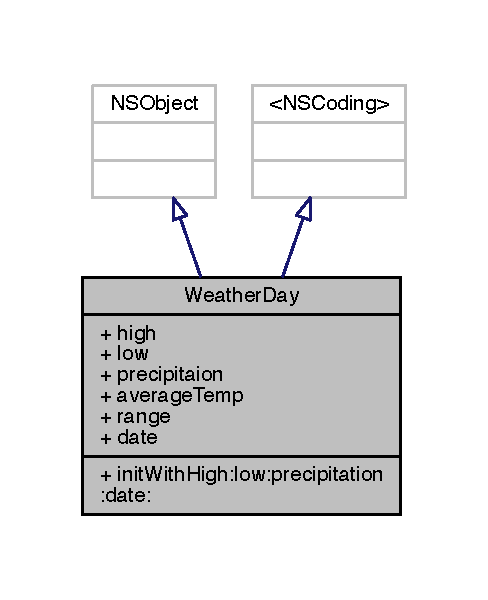
\includegraphics[width=234pt]{interface_weather_day__inherit__graph}
\end{center}
\end{figure}


Collaboration diagram for Weather\-Day\-:
\nopagebreak
\begin{figure}[H]
\begin{center}
\leavevmode
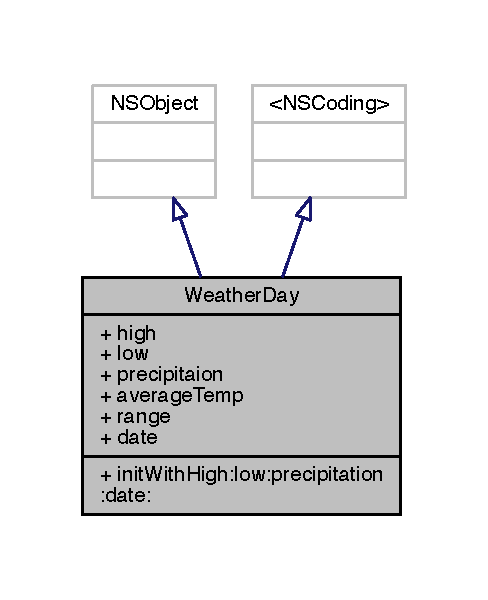
\includegraphics[width=234pt]{interface_weather_day__coll__graph}
\end{center}
\end{figure}
\subsection*{Instance Methods}
\begin{DoxyCompactItemize}
\item 
(instancetype) -\/ \hyperlink{interface_weather_day_a5a57d195f2f06cb96693b4b4d68fd955}{init\-With\-High\-:low\-:precipitation\-:date\-:}
\end{DoxyCompactItemize}
\subsection*{Properties}
\begin{DoxyCompactItemize}
\item 
N\-S\-Integer \hyperlink{interface_weather_day_a97d5aad192216fe0de9ebc43296cfb68}{high}
\item 
N\-S\-Integer \hyperlink{interface_weather_day_a677798c5423dabd4861214c5de4faf55}{low}
\item 
C\-G\-Float \hyperlink{interface_weather_day_a62a56a8c78976523287185d6dce106e1}{precipitaion}
\item 
N\-S\-Integer \hyperlink{interface_weather_day_a8447b6e2f7cd73dce25e53ae8ac4baaa}{weighted\-Average\-Temp}
\item 
N\-S\-Integer \hyperlink{interface_weather_day_ade050fc16334cf7cac350d222ff1a026}{range}
\item 
\hypertarget{interface_weather_day_a0217f0a16223b343331a1831eecd97bb}{N\-S\-Date $\ast$ {\bfseries date}}\label{interface_weather_day_a0217f0a16223b343331a1831eecd97bb}

\end{DoxyCompactItemize}


\subsection{Detailed Description}
Class representing a day's weather 

\subsection{Method Documentation}
\hypertarget{interface_weather_day_a5a57d195f2f06cb96693b4b4d68fd955}{\index{Weather\-Day@{Weather\-Day}!init\-With\-High\-:low\-:precipitation\-:date\-:@{init\-With\-High\-:low\-:precipitation\-:date\-:}}
\index{init\-With\-High\-:low\-:precipitation\-:date\-:@{init\-With\-High\-:low\-:precipitation\-:date\-:}!WeatherDay@{Weather\-Day}}
\subsubsection[{init\-With\-High\-:low\-:precipitation\-:date\-:}]{\setlength{\rightskip}{0pt plus 5cm}-\/ (instancetype) init\-With\-High\-: 
\begin{DoxyParamCaption}
\item[{(N\-S\-Integer)}]{high}
\item[{low:(N\-S\-Integer)}]{low}
\item[{precipitation:(C\-G\-Float)}]{prec}
\item[{date:(N\-S\-Date$\ast$)}]{date}
\end{DoxyParamCaption}
}}\label{interface_weather_day_a5a57d195f2f06cb96693b4b4d68fd955}
Initialize a new D\-Weather\-Day object 
\begin{DoxyParams}{Parameters}
{\em high} & The day's high \\
\hline
{\em low} & The day's low \\
\hline
{\em prec} & The days precipitation chance \\
\hline
\end{DoxyParams}


\subsection{Property Documentation}
\hypertarget{interface_weather_day_a97d5aad192216fe0de9ebc43296cfb68}{\index{Weather\-Day@{Weather\-Day}!high@{high}}
\index{high@{high}!WeatherDay@{Weather\-Day}}
\subsubsection[{high}]{\setlength{\rightskip}{0pt plus 5cm}-\/ (N\-S\-Integer) high\hspace{0.3cm}{\ttfamily [read]}, {\ttfamily [write]}, {\ttfamily [atomic]}}}\label{interface_weather_day_a97d5aad192216fe0de9ebc43296cfb68}
The day's high temperature \hypertarget{interface_weather_day_a677798c5423dabd4861214c5de4faf55}{\index{Weather\-Day@{Weather\-Day}!low@{low}}
\index{low@{low}!WeatherDay@{Weather\-Day}}
\subsubsection[{low}]{\setlength{\rightskip}{0pt plus 5cm}-\/ (N\-S\-Integer) low\hspace{0.3cm}{\ttfamily [read]}, {\ttfamily [write]}, {\ttfamily [atomic]}}}\label{interface_weather_day_a677798c5423dabd4861214c5de4faf55}
The day's low temperature \hypertarget{interface_weather_day_a62a56a8c78976523287185d6dce106e1}{\index{Weather\-Day@{Weather\-Day}!precipitaion@{precipitaion}}
\index{precipitaion@{precipitaion}!WeatherDay@{Weather\-Day}}
\subsubsection[{precipitaion}]{\setlength{\rightskip}{0pt plus 5cm}-\/ (C\-G\-Float) precipitaion\hspace{0.3cm}{\ttfamily [read]}, {\ttfamily [write]}, {\ttfamily [atomic]}}}\label{interface_weather_day_a62a56a8c78976523287185d6dce106e1}
The day's precipitation chance \hypertarget{interface_weather_day_ade050fc16334cf7cac350d222ff1a026}{\index{Weather\-Day@{Weather\-Day}!range@{range}}
\index{range@{range}!WeatherDay@{Weather\-Day}}
\subsubsection[{range}]{\setlength{\rightskip}{0pt plus 5cm}-\/ (N\-S\-Integer) range\hspace{0.3cm}{\ttfamily [read]}, {\ttfamily [write]}, {\ttfamily [nonatomic]}, {\ttfamily [assign]}}}\label{interface_weather_day_ade050fc16334cf7cac350d222ff1a026}
Custom getter \hypertarget{interface_weather_day_a8447b6e2f7cd73dce25e53ae8ac4baaa}{\index{Weather\-Day@{Weather\-Day}!weighted\-Average\-Temp@{weighted\-Average\-Temp}}
\index{weighted\-Average\-Temp@{weighted\-Average\-Temp}!WeatherDay@{Weather\-Day}}
\subsubsection[{weighted\-Average\-Temp}]{\setlength{\rightskip}{0pt plus 5cm}-\/ (N\-S\-Integer) weighted\-Average\-Temp\hspace{0.3cm}{\ttfamily [read]}, {\ttfamily [write]}, {\ttfamily [nonatomic]}, {\ttfamily [assign]}}}\label{interface_weather_day_a8447b6e2f7cd73dce25e53ae8ac4baaa}
Custom getter 

The documentation for this class was generated from the following files\-:\begin{DoxyCompactItemize}
\item 
Pack\-Manager/Weather\-Day.\-h\item 
Pack\-Manager/Weather\-Day.\-m\end{DoxyCompactItemize}

\hypertarget{interface_weather_report}{\section{Weather\-Report Class Reference}
\label{interface_weather_report}\index{Weather\-Report@{Weather\-Report}}
}


Inheritance diagram for Weather\-Report\-:\nopagebreak
\begin{figure}[H]
\begin{center}
\leavevmode
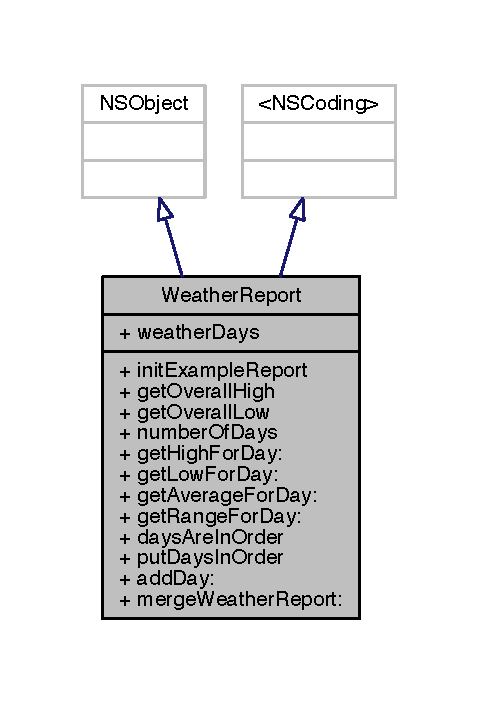
\includegraphics[width=174pt]{interface_weather_report__inherit__graph}
\end{center}
\end{figure}


Collaboration diagram for Weather\-Report\-:\nopagebreak
\begin{figure}[H]
\begin{center}
\leavevmode
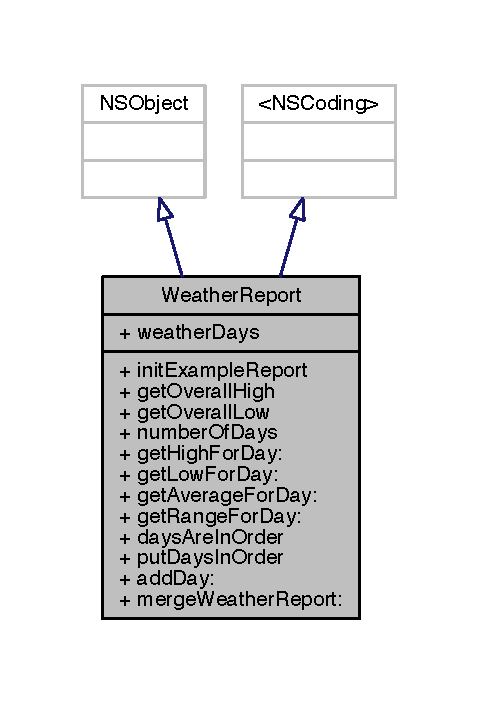
\includegraphics[width=174pt]{interface_weather_report__coll__graph}
\end{center}
\end{figure}
\subsection*{Instance Methods}
\begin{DoxyCompactItemize}
\item 
\hypertarget{interface_weather_report_aa6bbf5b779e0c4598e198adfeef73caa}{(N\-S\-Integer) -\/ {\bfseries get\-Overall\-High}}\label{interface_weather_report_aa6bbf5b779e0c4598e198adfeef73caa}

\item 
\hypertarget{interface_weather_report_a8044a91695febcfbd290533f0a2d7014}{(N\-S\-Integer) -\/ {\bfseries get\-Overall\-Low}}\label{interface_weather_report_a8044a91695febcfbd290533f0a2d7014}

\item 
\hypertarget{interface_weather_report_a43c87e18a2a90ba36e4426e066ec1bc0}{(N\-S\-Integer) -\/ {\bfseries number\-Of\-Days}}\label{interface_weather_report_a43c87e18a2a90ba36e4426e066ec1bc0}

\item 
\hypertarget{interface_weather_report_a2f163b73346d557e8e69f1ba4658fd6a}{(N\-S\-Integer) -\/ {\bfseries get\-High\-For\-Day\-:}}\label{interface_weather_report_a2f163b73346d557e8e69f1ba4658fd6a}

\item 
\hypertarget{interface_weather_report_a69f1a204d1941aeab765e2ca4bfd989c}{(N\-S\-Integer) -\/ {\bfseries get\-Low\-For\-Day\-:}}\label{interface_weather_report_a69f1a204d1941aeab765e2ca4bfd989c}

\end{DoxyCompactItemize}


The documentation for this class was generated from the following files\-:\begin{DoxyCompactItemize}
\item 
Pack\-Manager/Weather\-Report.\-h\item 
Pack\-Manager/Weather\-Report.\-m\end{DoxyCompactItemize}

\hypertarget{category_weather_report_07_08}{\section{Weather\-Report() Category Reference}
\label{category_weather_report_07_08}\index{Weather\-Report()@{Weather\-Report()}}
}


Collaboration diagram for Weather\-Report()\-:\nopagebreak
\begin{figure}[H]
\begin{center}
\leavevmode
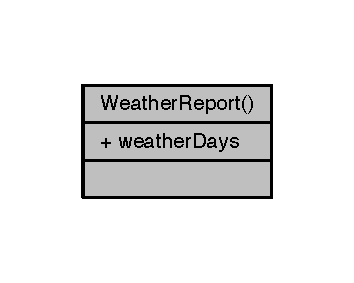
\includegraphics[width=170pt]{category_weather_report_07_08__coll__graph}
\end{center}
\end{figure}
\subsection*{Properties}
\begin{DoxyCompactItemize}
\item 
\hypertarget{category_weather_report_07_08_a87f6dd5f17905c87920e970633f67aa9}{N\-S\-Mutable\-Array $\ast$ {\bfseries weather\-Days}}\label{category_weather_report_07_08_a87f6dd5f17905c87920e970633f67aa9}

\end{DoxyCompactItemize}


The documentation for this category was generated from the following file\-:\begin{DoxyCompactItemize}
\item 
Pack\-Manager/Weather\-Report.\-m\end{DoxyCompactItemize}

\hypertarget{interface_weather_report_view_controller}{\section{Weather\-Report\-View\-Controller Class Reference}
\label{interface_weather_report_view_controller}\index{Weather\-Report\-View\-Controller@{Weather\-Report\-View\-Controller}}
}


Inheritance diagram for Weather\-Report\-View\-Controller\-:\nopagebreak
\begin{figure}[H]
\begin{center}
\leavevmode
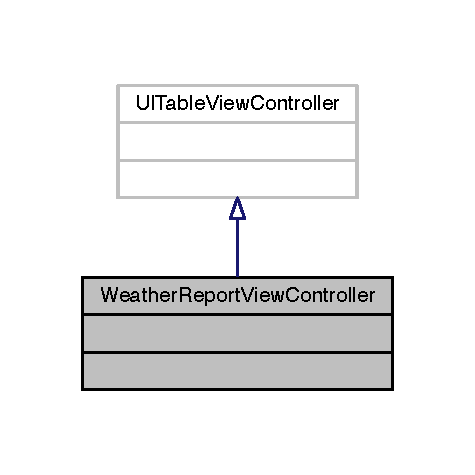
\includegraphics[width=228pt]{interface_weather_report_view_controller__inherit__graph}
\end{center}
\end{figure}


Collaboration diagram for Weather\-Report\-View\-Controller\-:
\nopagebreak
\begin{figure}[H]
\begin{center}
\leavevmode
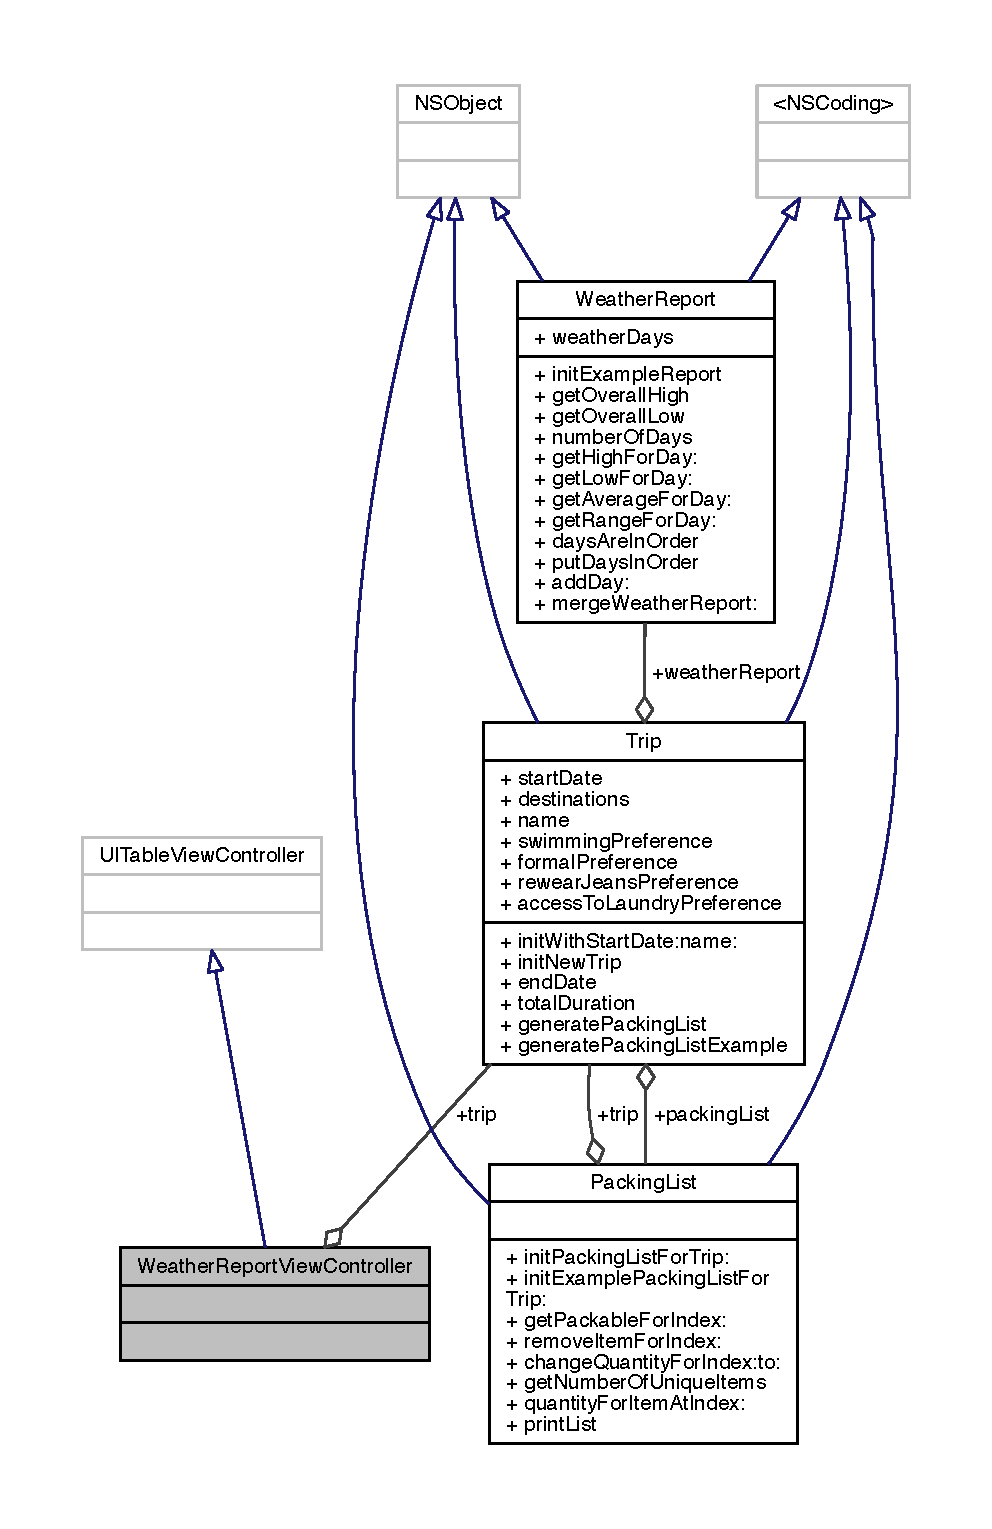
\includegraphics[width=350pt]{interface_weather_report_view_controller__coll__graph}
\end{center}
\end{figure}
\subsection*{Properties}
\begin{DoxyCompactItemize}
\item 
\hypertarget{interface_weather_report_view_controller_a0cf14329780feb3d74d5bf0da154ff21}{\hyperlink{interface_trip}{Trip} $\ast$ {\bfseries trip}}\label{interface_weather_report_view_controller_a0cf14329780feb3d74d5bf0da154ff21}

\end{DoxyCompactItemize}


The documentation for this class was generated from the following file\-:\begin{DoxyCompactItemize}
\item 
Pack\-Manager/Weather\-Report\-View\-Controller.\-h\end{DoxyCompactItemize}

\hypertarget{category_weather_report_view_controller_07_08}{\section{Weather\-Report\-View\-Controller() Category Reference}
\label{category_weather_report_view_controller_07_08}\index{Weather\-Report\-View\-Controller()@{Weather\-Report\-View\-Controller()}}
}


Collaboration diagram for Weather\-Report\-View\-Controller()\-:\nopagebreak
\begin{figure}[H]
\begin{center}
\leavevmode
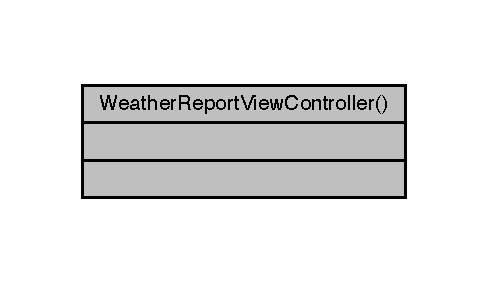
\includegraphics[width=234pt]{category_weather_report_view_controller_07_08__coll__graph}
\end{center}
\end{figure}


The documentation for this category was generated from the following file\-:\begin{DoxyCompactItemize}
\item 
Pack\-Manager/Weather\-Report\-View\-Controller.\-m\end{DoxyCompactItemize}

%--- End generated contents ---

% Index
\newpage
\phantomsection
\addcontentsline{toc}{chapter}{Index}
\printindex

\end{document}
